%%% The main file. It contains definitions of basic parameters and includes all other parts.

%% Settings for single-side (simplex) printing
% Margins: left 40mm, right 25mm, top and bottom 25mm
% (but beware, LaTeX adds 1in implicitly)
% \documentclass[12pt,a4paper]{report}
% \setlength\textwidth{145mm}
% \setlength\textheight{247mm}
% \setlength\oddsidemargin{15mm}
% \setlength\evensidemargin{15mm}
% \setlength\topmargin{0mm}
% \setlength\headsep{0mm}
% \setlength\headheight{0mm}
% \openright makes the following text appear on a right-hand page
% \let\openright=\clearpage

%% Settings for two-sided (duplex) printing
\documentclass[12pt,a4paper,twoside,openright]{report}
\setlength\textwidth{145mm}
\setlength\textheight{247mm}
\setlength\oddsidemargin{14.2mm}
\setlength\evensidemargin{0mm}
\setlength\topmargin{0mm}
\setlength\headsep{0mm}
\setlength\headheight{0mm}
\let\openright=\cleardoublepage

%% Generate PDF/A-2u
\usepackage[a-2u]{pdfx}

%% Character encoding: usually latin2, cp1250 or utf8:
\usepackage[utf8]{inputenc}

%% Prefer Latin Modern fonts
\usepackage{lmodern}
\usepackage{todonotes}
%% Further useful packages (included in most LaTeX distributions)
\usepackage{amsmath}        % extensions for typesetting of math
\usepackage{amsfonts}       % math fonts
\usepackage{amsthm}         % theorems, definitions, etc.
\usepackage{bbding}         % various symbols (squares, asterisks, scissors, ...)
\usepackage{bm}             % boldface symbols (\bm)
\usepackage{graphicx}       % embedding of pictures
\usepackage{fancyvrb}       % improved verbatim environment
\usepackage{natbib}         % citation style AUTHOR (YEAR), or AUTHOR [NUMBER]
\usepackage[nottoc]{tocbibind} % makes sure that bibliography and the lists
			    % of figures/tables are included in the table
			    % of contents
\usepackage{dcolumn}        % improved alignment of table columns
\usepackage{booktabs}       % improved horizontal lines in tables
\usepackage{paralist}       % improved enumerate and itemize
\usepackage[]{xcolor}  % typesetting in color
\usepackage{hyperref}
\usepackage[english]{babel}
\usepackage{float}
%%% Basic information on the thesis

% Thesis title in English (exactly as in the formal assignment)
\def\ThesisTitle{Similarity methods for music recommender systems}

% Author of the thesis
\def\ThesisAuthor{Michaela Vystrčilová}

% Year when the thesis is submitted
\def\YearSubmitted{2019}

% Name of the department or institute, where the work was officially assigned
% (according to the Organizational Structure of MFF UK in English,
% or a full name of a department outside MFF)
\def\Department{Department of Software Engineering}

% Is it a department (katedra), or an institute (ústav)?
\def\DeptType{Department}

% Thesis supervisor: name, surname and titles
\def\Supervisor{Mgr. Ladislav Peška, Ph.D.}

% Supervisor's department (again according to Organizational structure of MFF)
\def\SupervisorsDepartment{department}

% Study programme and specialization
\def\StudyProgramme{study programme}
\def\StudyBranch{study branch}

% An optional dedication: you can thank whomever you wish (your supervisor,
% consultant, a person who lent the software, etc.)
\def\Dedication{%
Dedication.
}

% Abstract (recommended length around 80-200 words; this is not a copy of your thesis assignment!)
\def\Abstract{%
Abstract.
}

% 3 to 5 keywords (recommended), each enclosed in curly braces
\def\Keywords{%
{music recommendation} {unsupervised feature extraction} {audio-based song similarity} {text-based song similarity}
}

%% The hyperref package for clickable links in PDF and also for storing
%% metadata to PDF (including the table of contents).
%% Most settings are pre-set by the pdfx package.
\hypersetup{unicode}
\hypersetup{breaklinks=true}

% Definitions of macros (see description inside)
\include{macros}

% Title page and various mandatory informational pages
\begin{document}
\include{title}

%%% A page with automatically generated table of contents of the bachelor thesis

\tableofcontents

%%% Each chapter is kept in a separate file
\chapter*{Introduction}\todo[inline]{LP:Spíše Abstract}
\addcontentsline{toc}{chapter}{Introduction}


\todo[inline]{LP:chápu myšlenku, ale chtělo by to ještě trochu zabrat na formulacích. Cílem práce není "introduce" ale spíše "compare". Možná by stálo začít něčím jako "The main focus of this thesis is the domain of song recommendation. This domain has several specific features such as... In this thesis, we primarily focus on comparison of existing methods for content-based song recommendation and implementing them in a web application.}
%\chapter{Introduction}

Millions of songs online provide an opportunity to find great songs for people with all kinds of music tastes. However, only a small fraction of the magnitude of all the songs produced becomes popular and those are the ones people are being exposed to the most. They are recommended to them on various platforms such as YouTube \footnote{https://www.youtube.com} or Spotify \footnote{https://www.spotify.com}, and played across all radio stations sometimes several times a day. After a while, older songs become less popular, one could use the term \textit{"overplayed"} and other (usually new) songs take their place. But what if a person's next favorite song already existed, it just did not become popular? It is unlikely to hear unpopular but possibly likeable songs for a person with unusual music preferences on the radio. Radio stations try to target as many listeners as possible. However with the assistance of a recommender collecting data about what a user listens to, it could help anyone discover tracks perfectly tailored for them without being dependant on their popularity.\\
The suggestions of recommendation systems for basically any online content is crucial. With the amount of songs as mentioned earlier but also movies, books, clothes, electronics and many more, it would be extremely time consuming for a person to go through all of it in order to find what they are looking for. Recommendation systems are trying to make it easier for people to find what they want for and even predict, what they will be looking for next or what they might want but maybe just do not know it yet. \\
There are three main method groups to generate (not only) music recommendations for users. First are collaborative-filtering methods (CF) where recommendations are based on like-minded users preferences, second are content-based methods where recommendations are based on the song content (tags, audio, lyrics, ...) and the third group are hybrid methods combining the first two together. \\
Generally, CF methods for all kinds of recommendation systems appear to be researched more extensively \cite{DBLP:journals/corr/abs-1712-07525} however, there are certain drawbacks these approaches. Most obviously, there is a problem with new, unrated songs because no user has viewed or liked them, so they cannot be recommended to like-minded users with a method based only on collaborative filtering. This is called the cold-start problem. Also, the recommendations tend to be dependent on user popularity patterns. Nevertheless, with enough user data, collaborative filtering methods generally outperform content-based methods \cite{van2013deep}. \\
Due to this, there are not many applications that would recommend songs based solely on their content and to the best of our knowledge there is no music recommendation application that would recommend songs to its users based only on lyrics. As this is a logical consequence of the findings above, we believe that a recommendation system based exclusively on content-based methods could be helpful for users with an unusual taste because collaborative filtering is popularity-dependant. Therefore the goal of this thesis to introduce such an application. \\
To create a content-based music recommender application we need to decide based on what content it will be recommending. A basic CB representation of songs is attribute-based. Attributes are the song's genre, the artist, creation year and so on. We are not using it in our application however because almost all music related application allow users to search based on tags. \\
We chose lyrics and audio as the content songs have to base the recommendations of the application on. Audio is something that every song has and it also is probably what is most important about it. People listen to music because it is a pleasant sound and it is likely that it is audio features that define, whether a person likes a song or not. \\
With lyrics it is a bit different. The main reason to study these methods is the lack of research for lyrics-based methods. There is an intuitive a notion that their performance might be doubtful, however, many studies evaluate them on their genre classification accuracy \cite{DBLP:journals/corr/Tsaptsinos17} or compare them to collaborative filtering systems \cite{Gossi2016LyricBasedMR} which does not always mimic actual user behaviour. \\
Recommendation is mostly based on similarity between items which can be defined in various ways. Both lyrics and audio need pre-processing before establishing similarity.  Because of that the goal of this thesis is to describe and test various ways of pre-processing text and audio in an unsupervised manner for content-based song similarity calculations, choose some of them based on previous studies and features, evaluate their performance on real user playlists, compare their performance and then implement chosen ones in a web application.\\

During our research it turned out that measuring song similarity based on lyrics and based on audio are two completely different tasks and there are multiple sub-problems in both approaches. Language, feature representation and similarity metrics for lyrics based methods and audio extraction, audio representation, feature extraction and similarity metrics for audio based similarity. We decided to focus on unsupervised learning of song feature representation which means encoding a song into a vector so that a standard similarity-based recommendation technique can be used to evaluate similarity of two arbitrary songs without having any information about genre or other tags. The vectors can also be used for more advanced algorithms using for example Recurrent neural networks to calculate similarity. That is however above the scope of this work. \\
The methods will be divided into two main groups. In the first one, songs will be encoded based on their lyrics in the second one based on audio. In both groups, we described basic as well as more advanced existing unsupervised learning encoding methods. We compare the text and audio recommendations based on these encoding methods but also compare methods within these two groups. \\
The web applications main purpose is to introduce the user to new songs he has not listened to yet based on a feature extraction method he chooses. The songs are provided by the applications default database but adding songs is possible too and their distance to other songs is taken into account for recommendations. \\

\todo[inline]{doted jsi nemluvila o zadne webove aplikaci ani o tom, ze by to melo byt cilem tve prace - je treba ten text logicky navazat. Celkove - nekde tady nejpozdeji by se mely objevit cile prace - pak na ne navazujes v dalsim textu bez toho, abys je tady explicitne zminila, coz je docela problem. Nekde tady je taky potreba zminit, ze zakladni mozne CB reprezentace songu je (attribute-based, ktery nepouzivame) text pisne a zvukovy zaznam, ale ze oboji je treba nejak predzpracovat predtim, nez se daji pouzit v doporucovani.}



\chapter{Data}

\section{Datasets}

\subsection{Lyrics dataset}
 We chose the \textit{55000+ Song Lyrics dataset} from Kaggle.com to obtain lyrics data. The Kaggle dataset originally contained 57 650 English songs. It’s lyrics are scraped from LyricsFreak. Extremely long and short lyrics were removed as well as all non-ASCII symbols from the lyrics. This is the dataset we used to train our text-based recommendation methods. Figure \ref{fig:lyrics_dataset} shows the first two entries of the dataset.\\
 \begin{figure}[h]
    \centering
	\includegraphics[height=60mm]{./img/dataset_preview.png}
	\caption{First two entries of the 55000+ Lyrics Dataset}
	\label{fig:lyrics_dataset}
\end{figure}

\subsection{User-information dataset}
To evaluate text and audio based methods on real-life user data, we had to select a dataset containing song information and lyrics as well as a dataset with information about users and their played tracks. First we tried to match the lyrics dataset onto the \textit{Echo Nest Taste Profile subset} from the Million Song Dataset website. However we only had 6800 songs with lyrics as well as user data.  We then tried the \textit{Thisismyjam} dataset also available on MSD. After removing songs we did not have lyrics for, we ended up with 16594 unique songs, and 45054 unique users. For each of the 16594 songs we also acquired a mono .wav file. \todo[inline]{Tady nevim, jestli mam rikat, ze jsem to stahla z YouTube, jestli je to jako v pohode}. \\

\section{Final dataset statistics}
Overall our final dataset had 160454 entries containing a user id, the artist, the song title and the lyrics. As our evaluation method is based on the users playlists (we took a portion of their played songs and tried to calculate the missing ones based on our metrics - will be described in more detail in the \textit{Experiment section}) we studied the dataset and especially the playlist length in more detail. //
Here are some important remarks:
\begin{itemize}
    \item Each user only has one playlist.
    \item We do not know, how many times a user played a song.
    \item We do not know which songs the user has played most recently.
    \item Users with only one song are useless for our evaluation.
    \item It should be easier to complete the dataset for users with longer datasets.
\end{itemize} 
When analyzing our dataset, it turned out, that out of 45054 users or lets say playlists, there are 22257 with only one song, which leaves us with 22797 we can use. Meaning, more than half of the playlists (about 51\% is useful for our evaluation as shown in figure \ref{fig:useless_users}.

The distribution of useful playlist lengths is shown in more detail in Figure \ref{fig:playlist_lenght_distribution}. We can see that most of the playlists are short, almost a third of them only contains two songs. The average number of songs per playlists (including those containing only one song) is 3.56. 
\begin{figure}[ht]
    \centering
	\includegraphics[height=110mm]{./img/playlist_description.png}
	\caption{The number of playlists for different lenghts}
	\label{fig:playlist_lenght_distribution}
\end{figure}
\todo{Tady mi to o 5 pisnicek nevychazi, takze to budu muset prepocitat, spis co rikate na tenhle graf? Pripadne jeste neco byste sem dodal?}

Each song has been played by 10.84 users on average. The distribution and the most popular songs are depicted in Figure \ref{fig:popular_song_distribution}. The by far most popular song with a total of 816 plays was \textit{Royals} by \textit{Lorde}. Second came \textit{Radioactive} by \textit{Imagine Dragons} with 674 users who played it. All other songs have been played by less than 500 users.

\begin{figure}[ht]
    \centering
	\includegraphics[height=80mm]{./img/popular_song_distribution.png}
	\caption{The number of playlists a song was in}
	\label{fig:popular_song_distribution}
\end{figure}

\chapter{Lyrics-based methods}\label{chap:lyrics_methods}
 In this chapter we will briefly describe some of the most prominent methods to represent songs based on their lyrics. After specifically focusing on the positive and negative aspects of these methods, we will select suitable candidates for testing and potentially for our web application.
 
 The reason to explore lyrics-based methods in this thesis is based on several factors. It is the belief of the authors that although the utilization of song lyrics is not completely unexplored as shown in Section \ref{sec:text_related_work}, there is space for innovative research. For example, to the best of our knowledge, there are no recommender systems that would rely solely on lyrics analysis. An advantage of these methods could lie in providing relevant recommendations that would be more variable compared recommendations from other, more traditional techniques.

\section{Text embedding methods}
\subsection{Bag of Words}
The Bag of Words commonly referred to as BoW is a text representation method which counts how many times a word appears in a document. In the context of this thesis, it counts, how many times a word appears in the song lyrics.
BoW represents each text (song) as a word-count vector where each index corresponds to the number of times a certain word appeared in it. An advantage of this encoding is its simplicity. The simplicity, however, brings some drawbacks. It for example ignores the fact that some words which can be found in most documents have a smaller informative value than others that only appear in a small fraction of the documents. 

\subsection{Tf-idf}
Term Frequency-Inverse Document Frequency is another way of transforming documents into vectors. Unlike the BoW, Tf-idf does not measure only the counts of words in a document but it also measures their relevance. As can be deduced from the title term frequency, first the number of appearances of a word $t$ in each document $d$ proportional to the number of all words in that document - \textit{tf(t,d)} - is computed. Then comes the inverse document frequency part - \textit{idf} - where the words are weighted as seen in Formula \ref{eq:idf}. The words that appear frequently in most documents have lower weights than those who only appear in some.

\begin{equation}\label{eq:idf}
idf(t) = log\frac{1+n_d}{1+df(t)} + 1
\end{equation}

Formula \ref{eq:tf_idf} is then the final Tf-idf formula multiplying the word frequencies with their weights:

\begin{equation}\label{eq:tf_idf}
tf\textnormal{-}idf(t,d) = idf(t)*tf(t,d) 
\end{equation}
In both of the formulas above \textit{t} is the word \textit{d} is the document $ df(t) $ is the number of documents containing the word \textit{t} and \textit{n\textsubscript{d}} is the total number of documents. 

\subsection{Word2Vec}
Word2Vec is a two-layer neural network trained to encode the linguistic context of a word introduced by Tomas Mikolov \cite{DBLP:journals/corr/abs-1301-3781}. Each word has an assigned vector in a vector space of typically hundreds of dimensions generated from a large corpus. The position of a word corresponds to its context, meaning, that words that share common context are closer to each other.

There are two possible Word2Vec architectures, the continuous bag-of-words (CBOW) and the continuous skip gram. The CBOW predicts the current word from the words surrounding it --- the context. It does not keep the order of the surrounding context words. The skip gram does, which makes it slower but also more effective, especially for infrequent words \cite{DBLP:journals/corr/abs-1301-3781}. The Skip-Gram architecture takes one word and predicts all the context around it.
\begin{figure}[h]
    \centering
	\includegraphics[height=70mm]{./img/cbow_skipgram_w2v_architecture.png}
	\caption{The CBOW and Skip-gram Word2Vec architectures from \cite{phdthesis}}
	\label{fig:cbow_skipgram_w2v_architecture}
\end{figure}


Multiple things have to be taken into account when training a W2V model. The information value of words that occur in all training documents is quite low so they can be removed to increase training speed. The dimensionality of the space also elevates accuracy only to a certain point so some threshold has to be set. Another parameter is the context window, which determines, how many words before and after a given word are included as its context.

\subsection{Doc2Vec}
Doc2Vec is an unsupervised algorithm that learns the feature representation of texts with varying lengths and encodes them into vectors of the same length. As the name suggests it is heavily based on the idea of Word2Vec. It was also first presented by the same group of researches in this paper \cite{DBLP:journals/corr/LeM14}. The main idea of the method is to use the Word2Vec model but add one more vector to represent the paragraph as a whole. As in the Word2Vec model, there are two architectures for the Doc2Vec approach. The Distributed Memory (DM) version of Paragraph vector and the Distributed Bag of Words (DBOW) version of the Paragraph vector. The DBOW is faster but does not consider the order of the words as it predicts a random group of words from the paragraph vector. The DM on the other hand takes previous words and the paragraph vector into account and predicts just one word. This way, because the paragraph does not shift across the text, the DM architecture is able to capture some word order but it requires more time to be trained.
\begin{figure}[h]
    \centering
	\includegraphics[width=140mm]{./img/DV_DBOW_doc2vec_architectures.png}
	\caption{The Doc2Vec DM and DBOW architecture taken from \cite{DBLP:journals/corr/LeM14}}
	\label{fig:dbow_dm_d2v_architecture}
\end{figure}
\subsection{Self organizing maps}
A self organizing map (SOM) is a type of a neural network that learns how to reduce the dimension of input data in an unsupervised manner. SOMs were introduced by Teuvo Kohonen \cite{Kohonen1982}. They use competitive dimensionality reduction (meaning the nodes in the SOM network compete to get the right to respond to the input data) which is quite unusual for neural networks as they usually use backpropagation. The models that SOMs compute are (usually) two dimensional spaces of neurons (called \textit{codebook} vectors) where similar examples are close to each other and dissimilar examples further from each other.

The SOM network is trained through an iterative process which is visualized in Figure \ref{fig:som_training}. It chooses one sample \textbf{x} \( \in R^n \) from the input training set at random and teaches it to itself. During teaching, the network feeds the chosen sample into all its units. A winner unit is calculated based on a similarity measure (usually Euclidean distance) between \textbf{x} and the \textit{codebook} vectors. Finally the values of the network units are updated. The best-matching unit is moved a closer to \textbf{x} and so are all the topological neighbours of the best unit.

The neighbours are defined by a neighbourhood function. It decreases with time and decides how radical the change around the winner will be. There are multiple functions that can be used. One can use the Gaussian kernel around the winner, however this is quite computationally expensive. A good and more efficient function is sometimes called the \textit{"bubble"} function which is constant over the whole neighbourhood of the winner and zero elsewhere \cite{SOM_training}.

\begin{figure}[H]
\begin{minipage}{\textwidth}
    \centering
	\includegraphics[width=140mm]{./img/Somtraining.png}
	\caption[A visualization of the training used for SOM networks]{Visualization of the training algorithm used for SOM networks. The blue area represents the distribution of the data. The white dot is the randomly selected sample. On the left, the SOM network nodes are randomly spread accross the space. When finding a winner (middle) and its defined neighbourhood (the yellow area) the network moves towards the datapoint and eventually after repeated iterations spreads mimicking the distribution of the data (left). This image is taken from Wikipedia\footnotemark}
	\label{fig:som_training}
\end{minipage}
\end{figure}

\footnotetext{https://commons.wikimedia.org/wiki/File:Somtraining.svg}

\section{Related work}\label{sec:text_related_work}

 There are several papers on music recommendation based on lyrics. For example \cite{Gossi2016LyricBasedMR} has shown, that simple Tf-idf song embedding was 12.6 times more accurate then just random suggestions on the musiXmatch dataset\footnote{https://labrosa.ee.columbia.edu/millionsong/musixmatch}.  In \cite{inproceedings} the authors compared the Doc2Vec and the SOM algorithm using cosine similarity for vector aggregation on a dataset containing Hindi songs and found that in their experiments, the SOM outperforms Doc2Vec. Paper \cite{DBLP:journals/corr/Tsaptsinos17} even studies using intact lyrics as input for Recurrent (LSTM) and Hierarchical neural networks and evaluates it based on genre classification.

\section{Text representation choices}
When choosing methods for our web application there are several factors to consider. Besides the expected accuracy of the algorithms, which is often difficult to estimate since lyrics-based recommendation methods have not been researched extensively, we have to consider the implementation as well as temporal complexity features of all the methods. Also, the fact that we want to focus more on a cross-sectional approach rather than a thorough optimization of one particular algorithm means, we prefer diversity in our chosen algorithms.  \\

The Bag of Words representation could be a good choice to get some kind of baseline results. Nevertheless, since the Tf-idf algorithm is widely based on the BoW and is still quite simple, we choose \textbf{Tf-idf} as our baseline. As mentioned at the beginning of this chapter, it was shown to be 12.6 times more accurate on the musiXmatch Dataset (MXD)\footnote{https://labrosa.ee.columbia.edu/millionsong/musixmatch} than just random suggestions, and that is what we hope to achieve with all of our text methods. A downside of the Tf-idf method is the length of its vectors. Even though they consist mostly of zeros, for our dataset, the length of each of them is over 40,000. 

Word2Vec and Doc2Vec are two similar approaches. The issue with Word2Vec when representing a whole document, in our case the lyrics for one song, is the transition between the word vectors and the whole document encoding. A commonly used aggregation method is to define the document vector as the mean of all the word vectors. 

Doc2Vec does not suffer from this problem, as its default is suited to represent a complete text. However, the problem with Doc2Vec is the amount of data it needs for training. Because every document is one sample, the number of documents necessary to achieve reasonable results is much higher than for Word2Vec where one sample is one word. What is also convenient with Word2Vec is, that there already exists a pre-trained Word2Vec model from Google\footnote{https://code.google.com/archive/p/word2vec/}. It consists of 3 million words with a 300-dimensional vector for each. Three hundred dimensions is a reasonable number (especially considering the fact that the Tf-idf vectors have over 40,000 dimensions). It was trained on roughly a billion words from a Google News dataset. Therefore we chose the \textbf{Word2Vec} method over the Doc2Vec.  

We also decided to implement the \textbf{SOM} network rather than Doc2Vec to represent songs because of a study showing, that Self organizing maps perform better than a Doc2Vec-based algorithm \cite{inproceedings}. It also does not need as much data as the Doc2Vec to be trained. 

One more thing we had to chose for the SOM was the form of the input. We decided to try the W2V representation. Mainly because the training of a self organizing map is quite computationally expensive and having vectors with over 40,000 dimensions would make it extremely time-consuming. We did not give up on the Tf-idf representation though. We trained another SOM where used Tf-idf vectors pre-processed by PCA which were reduced to length 4,457. 


\chapter{Audio-based methods}\label{chap:audio_methods}
In this section we will describe the possibilities of how to transform an audio signal (in our case from a .wav file) into representations suitable for song similarity calculations. This process consists of many steps and a lot of research has been done on all of them as illustrated in Section \ref{sec:audio_related_work}. \\
The reason we are focusing on audio in this thesis is the notion, that what people care about in a song is its sound. There are patterns in music that are pleasant to the human auditory system, otherwise, music would not be so popular. We believe it is the sound wave that contains these patterns. It is difficult to define what exactly they are so we hope that with the use of unsupervised machine learning algorithms, we will be able to find these them and then locate them in unseen songs as well. \\

Figure \ref{fig:audio_extraction} illustrates the steps of audio extraction. The blue part of the diagram describes the steps that are taken to acquire various basic music representations which are explained in Section \ref{sec:basic_music_representation_methods}. Each of these representations can be given as input to a machine learning algorithm as depicted in green from Section \ref{sec:audio_machine_learning} or deep learning algorithm from Section \ref{sec:audio_deep_learning} depicted in purple which both yield a final vector representation of the song. \\

\begin{figure}[h!]
    \centering
	\includegraphics[width=140mm]{./img/audio_feature_extraction_steps.png}
	\caption{A diagram displaying the steps taken in audio extraction. ML stands for machine learning and DL for deep learning.}
	\label{fig:audio_extraction}
\end{figure}

\section{Basic audio representation methods}\label{sec:basic_music_representation_methods}
 

\subsection{Raw waveform}
Sound is as vibration that spreads through gas, liquid or solid as a wave of pressure. For humans, the sound we hear has a frequency between 20Hz and 20kHz. Other sound waves are inaudible for humans. The most basic representation of sound as an audio signal is a \textit{waveform}. It captures the variation of pressure over time. As we cannot store infinite data to capture the state of the wave in every moment, we need to establish a sample rate. The sample rate is the number of samples per second at which the pressure is recorded as amplitude. Common sample rates are 44,100 Hz and 22,050 Hz that capture oscillation up to 22,050 Hz and 11,025Hz \cite{Schluter2017}.

\subsection{Spectrograms}
Raw waveform data have a lot of data points which makes them spaciously demanding. Luckily, they also display strong regularities in their oscillations which gives us a different, more compact possibility to represent audio signal. It encodes the signal as the strength of oscillations at various frequencies as opposed to amplitudes over time. Such an encoding is called a \textit{spectrum} when sinusoids are used as prototypical oscillations.
The spectrum is obtained from a waveform by applying \textit{Discrete Fourier Transformation}. The signal after DFT is represented by oscillations of a few frequencies spanning the full signal. \\
However a problem with this approach is, that for longer recordings, many oscillations are present only over some limited time span or change frequency. To represent all the oscillations the \textit{Short-Time Fourier Transformation} can be computed. It slices the audio into small often overlapping windows, computes their spectra and then puts them together in a chronological order. This spectra matrix is called the \textit{spectrogram} and for the song 'Someone Like You' by 'Adele' it has the shape of (2206, 7796). It can be visualized as a graph with frequency on one axis and time on the other axis. The intensity of a frequency is represented by color.

\begin{figure}[h!]
    \centering
	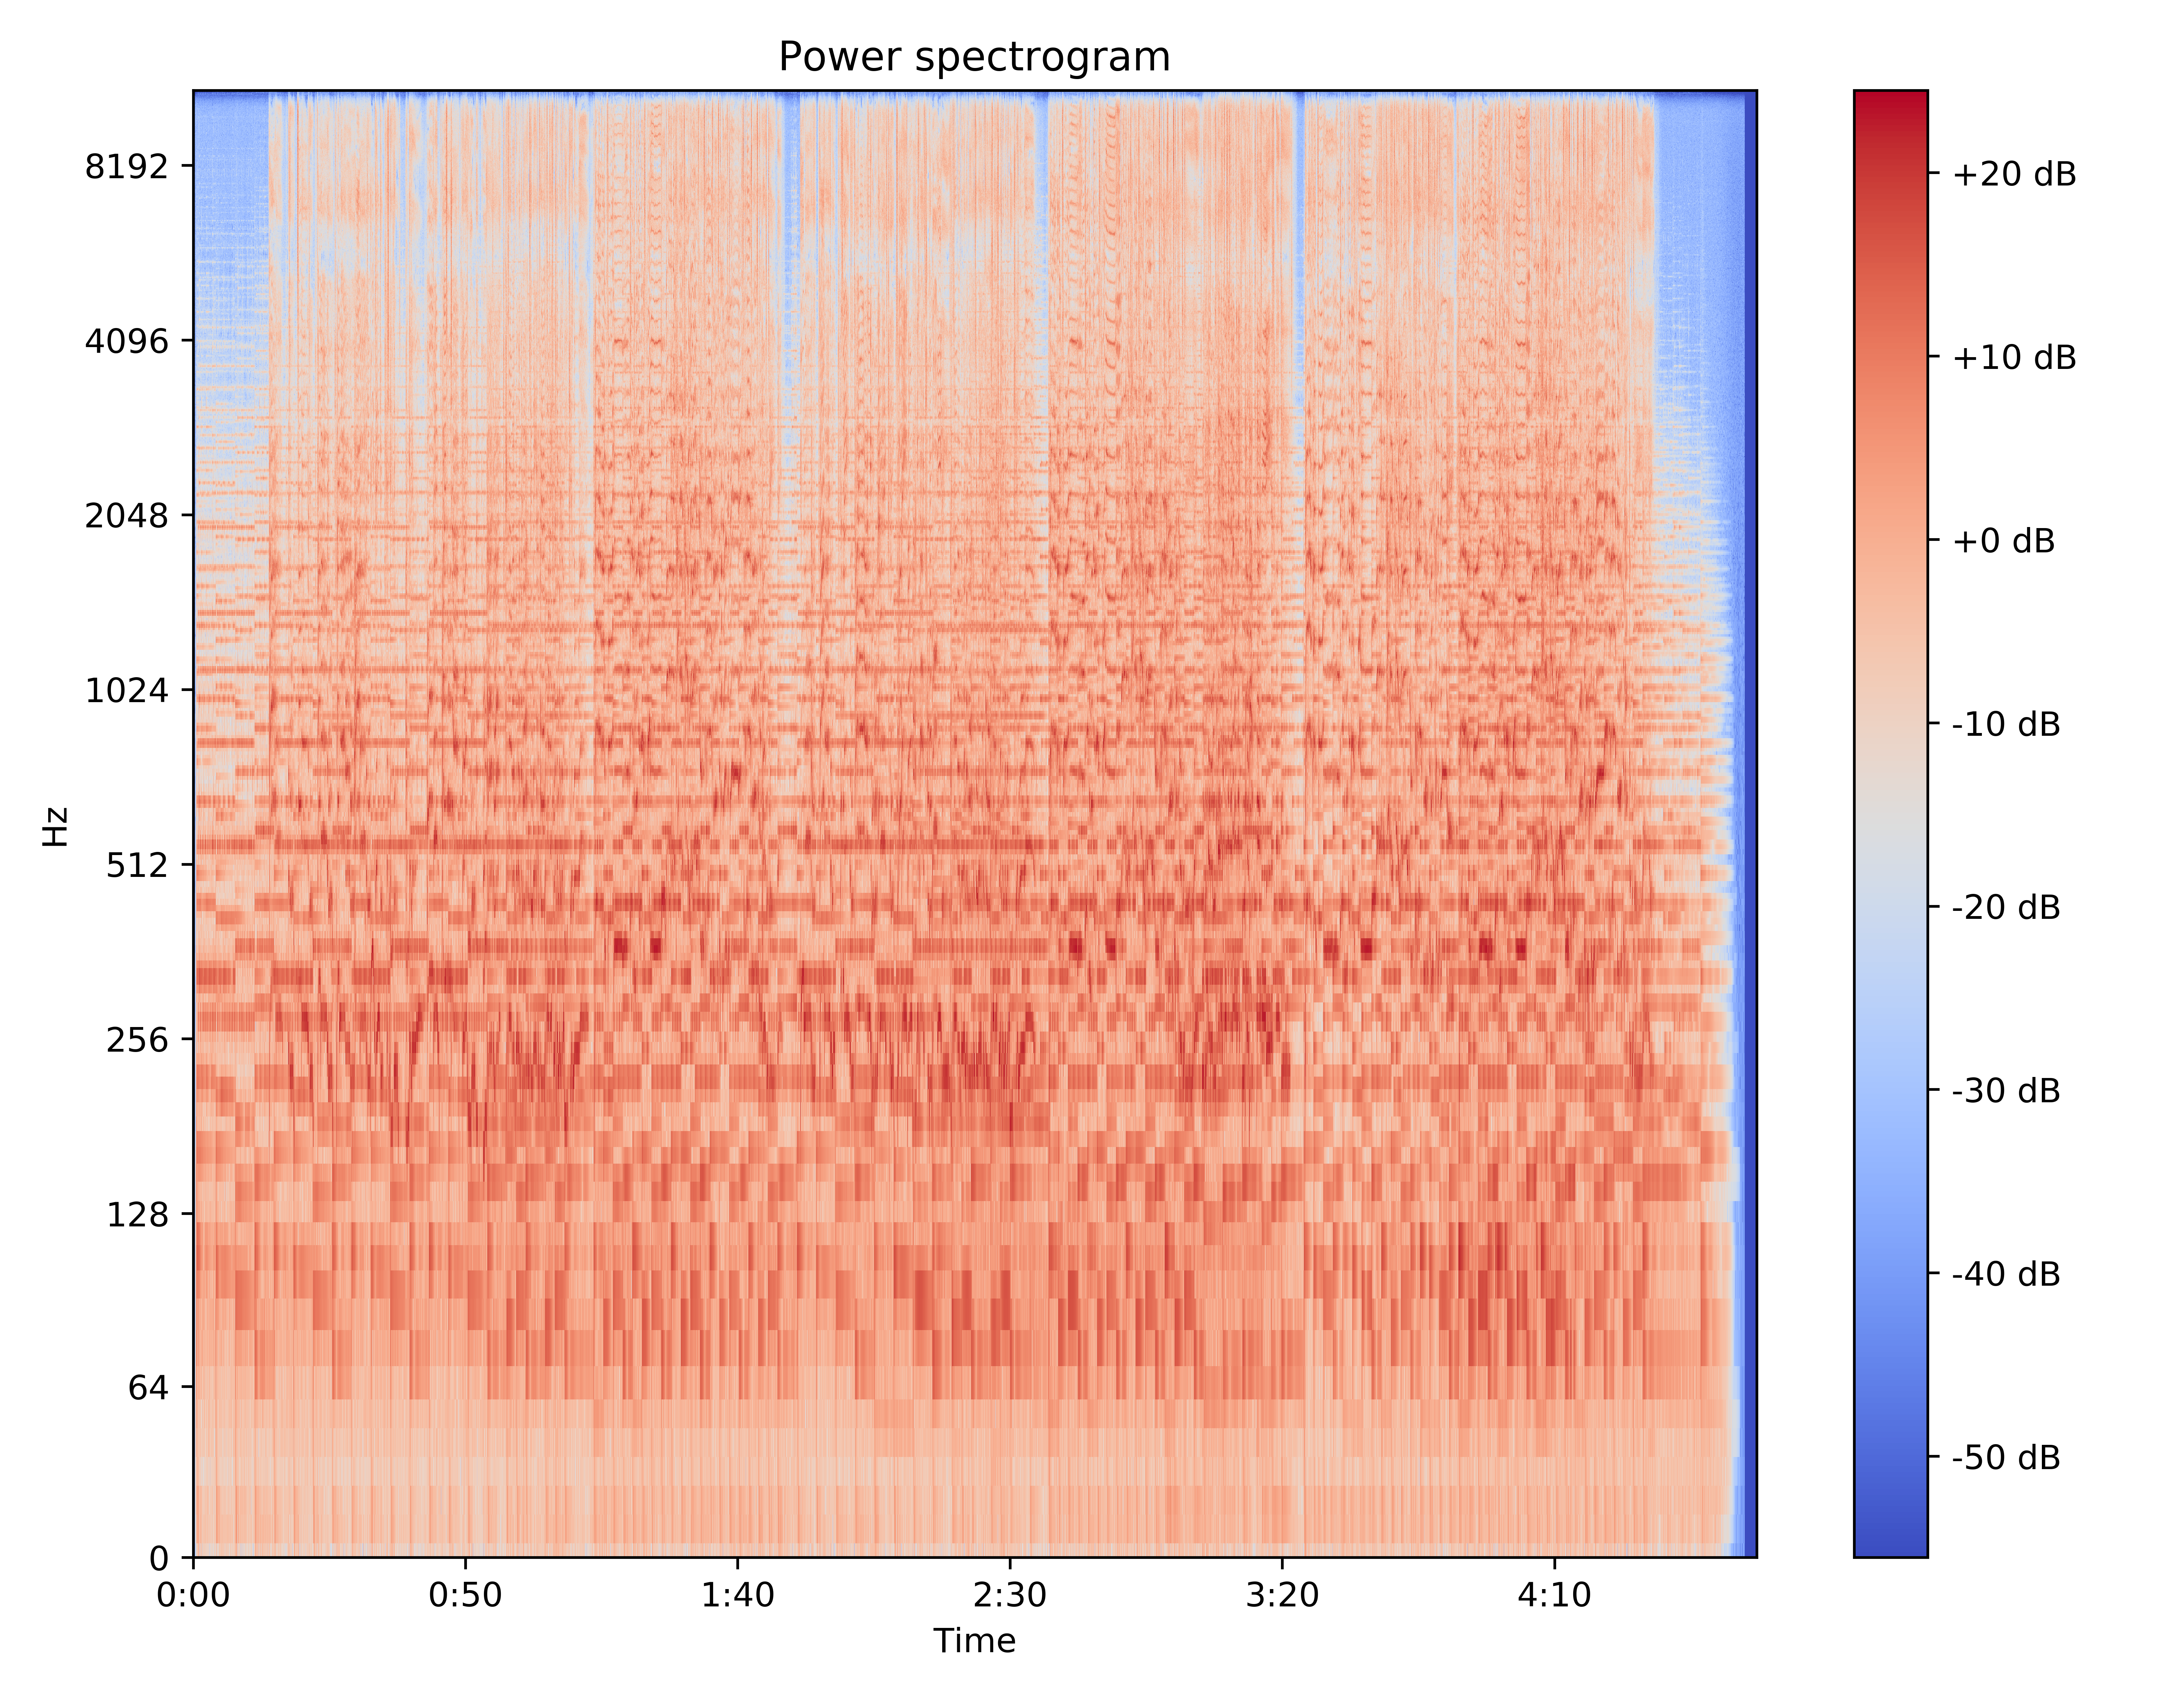
\includegraphics[width=140mm]{./img/spectrogram.png}
	\caption{Spectrogram of the song 'Someone Like You' by 'Adele'. The intensity of different frequencies over time is converted to decibels.}
	\label{fig:ilustrative_specrogram}
\end{figure}


\subsection{Mel Spectrograms}\label{ssec:mel_spectrograms_intro}
Mel-spectrograms are another approach to reducing the dimensionality of our data. However they are not mathematically based reductions of any kind of feature space. They are filtered spectrograms. Frequency bands are extracted by applying triangular \textit{Mel scale} filters to the power spectrum. The \textit{mel scale} after which this the spectrograms are called was named in 1937 in a study \cite{1937ASAJ....8..185S} by Volkmann and Newman. Since then it has been re-formulated multiple times, for example in \cite{mel_scale_fit} by Umesh at al. It is based on the human perception of pitch and loudness and allows us to convert from Hz to Mels. Mels which are more discriminatory at lower frequencies and less at higher frequencies - as is the human ear. \\
Each of the triangular filters has a response going from 1 to 0. They respond 1 at the center of some frequency and then their response decreases linearly to 0 towards to the place where they meet the neighbouring filters. When these filters are applied to a spectrogram, we get a mel-spectrogram. It is again a matrix of a smaller shape this time (320, 7796) for 'Someone Like You' and it can also be visualized as illustrated in Figure \ref{fig:ilustrative_melspecrogram}.

\begin{figure}[h!]
    \centering
	\includegraphics[width=140mm]{./img/melspectrogram.png}
	\caption{Mel-spectrogram of the song 'Someone Like You' by 'Adele'. The intensity of different frequencies over time is converted to decibels.}
	\label{fig:ilustrative_melspecrogram}
\end{figure}

\subsection{Mel Frequency Ceptral Coefficients}
Mel-Frequency Ceptral Coefficients (MFCC) are another step further in extracting audio features. They are obtained by applying \textit{Discrete cosine transformation} to mel-spectrograms. The DCT yield an even more compressed representation of them. For the song 'Someone Like You' by 'Adele' which we used as an example for spectrograms as well as mel-spectrograms, it created a matrix of shape (128, 7796) which looks as Figure \ref{fig:ilustrative_mfccs} illustrates.\\

A nice introcution to music signal processing with respect to deep machine learning, where spectrograms, mel-spectrograms and MFCCs are explained in more detail can be found here \cite{Schluter2017} where we also drew a lot of our information from.

\begin{figure}[h!]
    \centering
	\includegraphics[width=140mm]{./img/mfccs.png}
	\caption{MFCCs of the song 'Someone Like You' by 'Adele'. The intensity of different frequencies over time is converted to decibels.}
	\label{fig:ilustrative_mfccs}
\end{figure}

\section{Simple audio representation methods}\label{sec:audio_machine_learning}

\subsection{PCA}
PCA is a common machine learning algorithm used to reduce dimensionality of the feature space. It tries to keep features with most variance and discards feature in which all the data points are highly correlated. The data space is transformed in such a way, that the first principal component (PC) has the largest possible variance, the second PC the second largest variance etc. \\
Mathematically it is a orthogonal linear transformation to a new coordinate system where the base vectors are the principal components. To achieve this, we first need to center the data around the origin. That is done by subtracting the mean of each variable from the data. After that a covariance matrix is computed with its eigenvalues and corresponding eigenvectors. After normalizing the eigenvectors, they can be interpreted as a new basis vector. This new basis transforms the covariance matrix so that it becomes diagonal. Each of the diagonal elements represents the variance of each axis. All the components without any reduction give us the whole information about the input data, only in a vector space with a different basis. Every component explains some portion of the data's variance. The variance can be calculated by dividing every eigenvalue corresponding to an eigenvector with the sum of all eigenvalues. The dimensionality reduction is dependant on how many components we want. If we want to visualize the input data in a 2D graph, we create a space with only the first two PCs as a base and map all the data onto it. The reason to use this algorithm in our thesis is be mainly to reduce the length of the audio flattened audio matrices. \\
The PCA assumes that there is linear correlation between features. If there is not, the PCA will not discover it and will loose a lot of information with the dimensionality reduction it performs.

\section{Deep audio representation methods}\label{sec:audio_deep_learning}

\subsection{Convolutional neural networks}
Convolutional neural networks are neural networks that have become extensively researched after AlexNet (a form of CNN) was demonstrated in 2012 and outperformed all other methods for visual classification \cite{Krizhevsky:2012:ICD:2999134.2999257}. As with other neural networks, CNN's biggest advantage is to emulate behavior of unknown non-linear functions. CNNs have the ability to map high-dimensional data into a space of finite categories (with hundreds or thousands of classes). They are mostly used in visual imagery tasks. \\
The idea behind convolutional neural networks is to use \textit{local filters} instead of creating fully connected layers. This has risen from the idea that in images, there are correlated compositions on short scale distances, rather than at large distances. For example when detecting a human face in an image with a tree in the background, the tree does not have much to say about the face, unlike the eyes or the nose by which the face can be identified and are in a much greater proximity to each other. This is also the reason why in the CNN's architecture, the layers are not fully connected. \\
There are 4 main components that are generally be included in every CNN network. The \textit{Convolution layer},the \textit{ReLU}, the \textit{Maxpooling layer} and the \textit{Fully connected layer} that yields the output. To briefly describe these layers lets start with convolution. The convolutional layer helps to reduce the number of connections and weights. It consists of filters that can be learned. These only take a small number of nearby features into account at a time but extend through the whole input. Each of the filters crates a 2D activation map by computing the dot product of entries of the filter and the input. ReLU (rectified linear unit) is generally used to increase non linear properties of the decision function. Its function is $ f(x) = max(0,x) $ which is applied to the results of the convolution to speed up training --- compared to previously used functions for example sigmoid functions --- without affecting the receptive fields of the convolution layer. The pooling layer also reduces the number of parameters and helps prevent over-fitting. The most common function to implement is \textit{max pooling}. The features are partitioned into a set of non-overlapping rectangles (if input is 2D) and each of these rectangles  is represented by its maximal value. 
The final layer is usually a fully connected. Its neurons have connections to all activations of the previous layer and their activation is then computed as an affine transformation. 

\subsection{Deep belief networks}
Deep belief networks introduced by Hinton \cite{Hinton504} are multiple \textit{Restricted Boltzmann machines} greedily stacked on top of each other. RBMs are shallow two-layer neural nets created by Paul Smolensky in 1986 \cite{Smolensky1986InformationPI}. The first layes is called the visible layer, the second layer is called the hidden layer. The nodes of each layer communicate with the previous and subsequent layer but there are no connections between nodes of the same layer. Each visible node takes a low level feature to be learned and multiplies it by some weight. The results for each feature of an input sample are then summed, bias is added and this is the result passed through and activation algorithm which produces an output for each hidden node. These outputs then can be redirected into another hidden layer instead of the output of the neural network. \\
RBMs also have the ability to reconstruct data without supervision. When the input makes it through both layers it then becomes input for the hidden layer and travels through the neural network in the opposite direction. The activations are multiplied by the same weights and passed to the visible layer where a new bias is added. The output of the visible layer is then compared to the initial input and the network adjusts weights so that it minimizes the difference between the input and the output.

\subsection{Recurrent neural networks}
Recurrent neural networks have one major difference compared to other neural networks. They include feedback loops in their structure which allows them to exhibit dynamic behaviour and makes them useful for processing sequential data. RNNs have a hidden state that is determined by previous states and is updated with every subsequent step. There are many variants of RNNs such as \textit{Fully recurrent, Long short-term memory} introduced by Hochreiter and Schmidhuber in \cite{doi:10.1162/neco.1997.9.8.1735}, \textit{Gated recurent units} first described in \cite{cho-etal-2014-learning}, or \textit{Bi-directional} invented by Schuster and Paliwal in \cite{Schuster1997BidirectionalRN}. \\
Recurrent neural networks are used for working with sequential data for example in speech recognition \cite{DBLP:journals/corr/abs-1303-5778} or time-series anomaly detection \cite{inproceedings_RNN_anomaly_detection}.


\subsection{Autoencoders}
Autoencoders are not tied to one type of neural network. They can be build from recurrent layers, convolutional layers or using a simple Multi-layer Perceptron.\\
The autoencoder has two parts the encoder and the decoder. It is trained in an unsupervised manner. The encoder takes the input data and reduces its dimensions. The decoder then tries to recreate it into its original form without knowing, what the data looked like before the encoder processed it. The idea is, that over time, the encoder learns how to shrink the data with retaining as much information as possible for the decoder so the decoder it is able to recreate the original form as accurately as possible. 

\section{Related work}\label{sec:audio_related_work}
For the signal representation, there is obviously the possibility to use raw audio data as input for any machine learning algorithm. This however is a quite uncommon approach and when tested recently in tag prediction \cite{6854950} it had worse results than standard spectrograms. Multiple studies and experiments have been done using spectrograms as audio representation for classification tasks --- for example \cite{wang2014improving} --- or for unsupervised learning \cite{van2013deep}, \cite{Ramakrishnan2017song2V}, \cite{NIPS2009_3674}, which is what also our area of interest. \\
In these studies the inputs were fed into various neural network. The output of those was then evaluated and compared to music classification or simply music similarity estimation using similarity measures directly on spectrograms. We are going to do a similar thing in this thesis. Our evaluation will be done on user playlists and the methods will be compared to each other.

\section{Audio implementation choices}

\subsection{Basic audio representation choices}
At first when developing the web application we had the hope of using at least some of the raw data representation, to build some sort of base-line model. However, this turned out to be quite difficult as the vectors from flattened spectrograms, mel-spectrograms and mfccs have tens sometimes even hundreds of thousands of features. Therefore, although we implemented and evaluated recommendations based on mel spectrograms and mfccs, to include them in the proposed web application turned out to be too time consuming. The specific reasons are described in more detail in Chapter \ref{chap:experiments}. For the application, only PCA transformed mel-spectrograms and MFCCs were selected as they have a significantly reduced number of dimensions.


\subsection{Deep Audio representation choices}
Neural networks are a quickly developing and expanding field with many various applications. It is difficult to build an accurate neural network for specific task even with experience in deep machine learning. Because that is not what we have, we chose our neural network architecture and parameters based on literature relevant to the topic of audio-based music recommendation. The main requirements we had for our algorithms was that they have to work in an unsupervised manner and that they have to reduce the feature space. This pruned the number of possibilities for us considerably, as most architectures are designed for music classification (mostly into genres) or speech and sound recognition. \\
We decided that autoencoders suite our task in this thesis best. It is an unsupervised algorithm, with the task is to encode the input sample into a smaller dimension which is exactly what the encoder part does. The decoder transforms it again into the same vector however, this part of the autoencoder is only necessary for training.\\
Since we are working with sound data, the choice was to use RNN layers which have the ability to encode sequences (spectrograms, mel-spectrograms and mfccs are 2D matrices). These choices were mainly inspired by this paper \cite{inproceedings_RNNs}. However we want to add more methods into comparison, so we implemented not only neural networks with GRU layers but also LSTM layers and used spectrograms, mel-spectrograms and also mfccs as input rather than focusing on one type of layer, input and tuning one particular neural network to give the best results possible. 
\chapter{Experiments}\label{chap:experiments}

In this chapter we describe the experiments we performed on song preprocessing methods chosen in Chapters \ref{chap:lyrics_methods} and \ref{chap:audio_methods}. This includes describing every method's input, training (if there was any) and output (meaning the vector-encoded representations for each song in the SD). All this is presented in Sections \ref{sec:text_experiments}, \ref{sec:simple_audio_experiments} and \ref{sec:deep_audio_experiments}. Another thing we did not cover yet and will be presented here, in Section \ref{sec:similarity_metrics}, is describing how the different vector representations will be aggregated into a definition of similarity.

In Section \ref{sec:evaluation} we acquaint the reader with evaluation methods, the reasons we decided to use them and the evaluation results for each method. The results are first presented separately for each method (or a group of closely related methods) in Sections \ref{sec:text_results}, \ref{sec:simple_audio_resutls} and \ref{sec:deep_audio_results}, and then summarized and interpreted in Section \ref{sec:discussion} where various graphs and tables illustrating the prominent or interesting trends and tendencies can be found. Before all this however, we start with stating, what the expected outcomes were initially.

\section{Expectations}\label{sec:expectations}

Even before reading any literature, we made two main predictions: 
\begin{itemize}
    \item \textbf{First:} Audio-based methods will perform better than text-based methods.
    \item \textbf{Second:} More advanced methods will outperform simpler machine learning methods.
\end{itemize} 
By more advanced methods we mean methods that were invented more recently, are more computationally expensive and/or have a more complicated mathematical idea behind them. 

The first prediction was mostly based on the intuition, that audio contains more information about a song than the lyrics and it is also what people care about more when listening to music, both of which makes it more relevant for song encoding. 

The second prediction was also based on intuition and later supported by reading into this topic. Most of the papers we studied (meaning those in Sections \ref{sec:audio_related_work} and \ref{sec:text_related_work}) were describing neural networks performing audio or text-based recommendation or classification. Their results were then compared to simpler algorithms which they mostly outperformed. 

\section{Experimentation protocol}
Every method was trained on either lyrical or audio data of all 16,594 songs from the SD dataset.
For each method (except of raw audio methods which do not need any), we created a model. In addition, we created a matrix --- the \textit{Representation matrix}, denoted as  $R_m$ where $m$ stands for a particular method ---  after training the method's model. Each $R_m$ has the shape of ($16594$ x $l(v_m) $) where $l(v_m)$ is the length of the song vector representation for method $m$. Row $R_{m_{i,*}}$ contains the representation of song $s_i$ from the SD dataset using method $m$. 

We also calculated a \textit{Distance matrix} denoted as $D_m$ for every method. The shape of the $D_m$ is ($16594 $ x $ 16594$) and it is the same regardless of the method. On position $D_{m_{i,j}}$ is the similarity of $R_{m_{i,*}}$ and $R_{m_{j,*}}$. We talk more about similarity in Section \ref{sec:similarity_metrics}. \\

To make things easier for the rest of the thesis we now present all the methods that were tested and introduce a nomenclature. There are 3 different
parts each method name has --- the name of the main algorithm, the name of the input and the length of the output vector. Every method can be uniquely 
identified by a combination of these three parts. Where there is only one or
two parts necessary to uniquely identify the method, we omit those parts which are surplus. \\
The tested methods are:
\renewcommand\labelitemii{\textperiodcentered}
\begin{itemize}
     \item \textbf{Tf-idf} which stands for the Tf-idf method. \\
        Training is described in \ref{ssec:TF_idf_experiments} and the results in \ref{ssec:tf_idf_results}.
    \item \textbf{PCA\_Tf-idf} which stands for PCA with Tf-idf vectors as input. \\
    Training is described in \ref{ssec:PCA_on_tf_idf_experiments} and the results in \ref{ssec:pca_tf-idf_results}.
    \item \textbf{W2V} which represents the Word2Vec method. \\
        The training is described in \ref{ssec:w2v_experiments} and the results in \ref{ssec:w2v_results}.
    \item \textbf{SOM\_PCA\_Tf-idf} and \textbf{SOM\_W2V} which stand for the SOM network with PCA\_Tf-idf vectors as input and the SOM network with W2V vectors as input. \\
            Training is described in \ref{ssec:som_experiments} and the results in \ref{ssec:som_results}.
    \item \textbf{Raw mels} which are raw mel-spectrograms. \\
             Training described in \ref{ssec:raw_mels_experiments} and the results in \ref{ssec:mel_results}.
    \item \textbf{Raw MFCCs} which are raw MFCCs. \\
        Training is described in \ref{ssec:raw_mfccs_experiments} and the results in \ref{ssec:raw_mfccs_results}
    \item \textbf{PCA\_spec\_1106} and \textbf{PCA\_spec\_320} which stand for PCA with spectrograms as input and output lengths of 1,106 for the first method and 320 for the second method. \\
        Training is described in \ref{ssec:PCA_spec_experiments} and the results in \ref{ssec:pca_spec_results}.
    \item \textbf{PCA\_mel\_5715} and \textbf{PCA\_mel\_320} which stand for the PCA with mel-spectrograms as input and the output length of 5,715 for the first method and 320 for the second method. \\
        Training is described in \ref{ssec:pca_mel_experiments} and the results in \ref{ssec:pca_mel_results}.
    \item \textbf{GRU\_spec\_20400} and \textbf{GRU\_spec\_5712} which stand for an autoencoder with GRU layers and spectrogram input. The output vectors have length 20,400 for the first method and 5,712 for the second method. \\
    The architecture is described in \ref{ssec:nn_architectures}, training is described in \ref{ssec:GRU_spec_experiments} and the results in \ref{ssec:gru_spec_results}.
    \item \textbf{LSTM\_spec\_20400} and \textbf{LSTM\_spec\_5712} which stand for an autoencoder with LSTM layers and spectrogram input. \\
        The architecture is described in \ref{ssec:nn_architectures}, training is described in \ref{ssec:LSTM_spec_experiments} and the results in \ref{ssec:LSTM_spec_results}.
    \item \textbf{GRU\_mel} which stands for an autoencoder with GRU layers and mel- spectrogram input. \\
        The architecture is described in \ref{ssec:nn_architectures}, training is described in \ref{ssec:GRU_LSTM_mel_experiments} and the results in \ref{ssec:GRU_LSTM_mel_results}.
    \item \textbf{LSTM\_mel} which stands for an autoencoder with LSTM layers and mel- spectrogram input. \\
    The architecture is described in \ref{ssec:nn_architectures}, training is described in \ref{ssec:GRU_LSTM_mel_experiments} and the results in \ref{ssec:GRU_LSTM_mel_results}.
    \item \textbf{GRU\_MFCC} which stands for an autoencoder network with GRU layers and MFCCs as input. \\
        The architecture is described in \ref{ssec:nn_architectures}, training is described in \ref{ssec:GRU_LSTM_MFCC_experiments} and the results in \ref{ssec:GRU_LSTM_MFCC_results}.
    \item \textbf{LSTM\_MFCC} which stands for an autoencoder with LSTM layers and MFCCs as input. \\
        The architecture is described in \ref{ssec:nn_architectures}, training is described in \ref{ssec:GRU_LSTM_MFCC_experiments} and the results in \ref{ssec:GRU_LSTM_MFCC_results}.

    
\end{itemize}

\section{Text method experiments}\label{sec:text_experiments}

\subsection{Tf-idf experiments}\label{ssec:TF_idf_experiments}

\subsubsection{Input}
The lyrics of each song from SD were stripped of all punctuation characters as well as apostrophes and converted into a single string. All lyric-strings were appended into a list of strings which formed the training dataset.
\subsubsection{Training}
The training dataset was given to the \texttt{fit\_transform} method as a parameter. The method was called on an instance of \texttt{TFidfVectorizer} from Python's \texttt{sklearn} package. The results were saved into the $R_{Tf-idf}$. The \texttt{TFidfVectorizer} instance was saved as the model to be potentially used in the proposed web application. 

\subsubsection{Output}
The song representations were vectors of length 40,165. They contained a lot of zeros so it was possible to store them as \textit{sparse vectors}. Sparse vectors however, are more difficult to operate with and therefore we also converted them into dense vectors.

\subsection{PCA on Tf-idf}\label{ssec:PCA_on_tf_idf_experiments}

Because simple Tf-idf yielded good results we wanted to implement it. The long vectors posed a problem to our web application though. It is sometimes necessary in the application to calculate the distance between a newly added song and all the songs that are already in the database and this calculation is more complex for longer vectors. To reduce the complexity of this task but still use Tf-idf we decided to try to reduce the dimensions of the vectors using PCA.

\subsubsection{Input}
As input, we provided the Tf-idf vectors for songs from SD to the PCA which we acquired as described \ref{ssec:TF_idf_experiments}. We did not normalize them.

\subsubsection{Training}
We first trained a PCA from Python's \texttt{sklearn.decomposition.PCA} without any dimensionality reduction. We then chose a space were the explained variance ratio was equal to 90\%. This space had 4,457 dimensions. Knowing this, we trained a new PCA instance with 4,457 components which reduced our Tf-idf vector's length from 40,165 to 4,457 and saved it as the model.

\subsubsection{Output}
The output were vectors of length 4457 and were saved to the $R_{PCA\_Tf-idf}$.

\subsection{Word2Vec experiments}\label{ssec:w2v_experiments}

\subsubsection{Input}
The input for the W2V model was the same as for the Tf-idf method.

\subsubsection{Training}
In the case of Word2Vec, we did not perform any training. Instead, we used the a subset of the pre-trained W2V model from Google\footnote{https://code.google.com/archive/p/word2vec/} containing 200,000 most common words which cover all meaningful words in the song lyrics we have. Most common means, that they appeared most in their training documents. If there was a word in a song that was not in the subset it was ignored. 

\subsubsection{Output}
Because the Google model takes always just one word as input and returns its vector of fixed length 300, we had to put the word vectors together into one song-representation vector. We chose a basic approach where we averaged all the word vectors into one final song vector. The song vector's position $i$ contained the average over the values of word vectors' position $i$. This approach yielded a vector of length 300 which is significantly lower than the Tf-idf vector.\\

\subsection{SOM experiments}\label{ssec:som_experiments}

\subsubsection{Input}
We tried the W2V vectors from \ref{ssec:w2v_experiments} as input for the self organizing map, mainly because of their length and also because we were hoping, that the SOM could improve the results of the W2V method. We also tried to train the SOM on the output vectors of the PCA\_Tf-idf method. We did not try the raw Tf-idf vectors as they are longer and it would prolong training significantly. Also, it makes sense to use PCA\_Tf-idf because it yielded better results than raw Tf-idf.

\subsubsection{Training}
We used a python library called \texttt{minisom} \cite{Vettigli2019} to create the self organizing maps. We build a map with a grid size $5*|SD|$ and the number of iterations was also 5 times the size of SD. We saved a model after each multiple of 16,594 iterations and interestingly, the representations did not change after 33,187 iterations (which is 2*16,594). It was also necessary to normalize the input vectors and set learning rate to 0.2. Otherwise the songs formed 3 to 5 large clusters on the grid placing thousands of songs on the same coordinate. 

\subsubsection{Output}
The output representation for each song was a vector of length two. It is possible to display the songs on a 2D map which we also did and it can be seen in Figure \ref{fig:som_map}. 

\section{Simple audio method experiments}\label{sec:simple_audio_experiments}

\subsection{Audio preparation}\label{ssec:audio_prep}

In order to encode audios of songs, we first needed to define some kind of standard audio-form to make the audio information suitable for the machine learning methods that we are testing in this section and the next. We decided to extract chunks of the same duration from all songs, so the input vectors for each category (spectrograms, mel-spectrograms and mfccs) are also of the same length within each category. Since all songs have different lengths and one complete 3.5 minute long song results in a spectrogram of size 5,214x2,206 which when flattened is a vector of length 11,502,084 we decided to extract only 15 second excerpts from each song to create spectrograms, mel-spectrograms and MFCCs from those. We took 5 seconds between the 15th and 20th second, 5 seconds starting in the middle of the song and 5 seconds starting 15 seconds before the end. We did not start at the beginning and at the end because in some songs, there is silence or applause or some talking before the actual song starts or after it ends. \\

It was also necessary to decide on some parameters for spectrogram, mel-spectrogram and MFCC extractions such as window width, window overlap and the number of mel-frequency bands. As stated previously, our neural networks were inspired by \cite{inproceedings_RNNs} where they also performed parameter optimisation for the mel-spectrograms which they used as input for neural networks. We decided to use the reported parameters to create the spectrograms, mel-spectrograms in this thesis. We use spectrograms, mel-spectrograms and MFCCs as input for not only neural networks but also the PCA.

The resulting choices were following. We set window width $w$ to 0.2 and window overlap $w_o$ to 0.5$w$ = 0.1. For mel-spectrograms it is also necessary to choose mel-frequency bands which were set to 320 because in the findings from \cite{inproceedings_RNNs}, the performance of neural networks did not increase for values higher than 320. For MFCCs we decided to set the number of coefficients to 320 which is the same as the number of Mel- frequency bands.

With these parameters, the shape of an extracted spectrogram was (408 x 2206) which is a vector of lenght 900,048 when flattened. A mel-spectrogram matrix had the shape of (408 x 320) which when flattened is 130,560 and the MFCC matrix had the shape of (646 x 128) which when flattened is a vector of length 82,688.

We used Python's \texttt{librosa} library \cite{brian_mcfee_2019_2564164} to cut songs into the 15 second excerpts which we then stored the in .wav files. We used methods \texttt{librosa.core.stft} to generate spectrograms \texttt{librosa.feature.mel\_spectrogram} to generate mel-spectrograms and for the MFCC coefficients we used \texttt{librosa.feature.mfcc} all of which received the 15 second audio excerpt from the .wav file loaded using \texttt{librosa.core.load} as a parameter. These functions return a matrix of shape ($m$ x $n$) where $m$ is the number of timestamps and $n$ the number of features. The reason why the MFCC matrix has a different number of timestamps than spectrograms and mel-spectrograms for the same length of audio is, that we only set the number of MFCCs in the \texttt{librosa.core.mfcc} function but left the window width and window overlap default.

\subsection{Raw Mel-spectrograms}\label{ssec:raw_mels_experiments}
The mel-spectrograms were created from the 15 second long audios described in \ref{ssec:audio_prep}. Extracting spectrograms respectively mel-spectrograms does not require any training. It a is mathematical procedure explained in \ref{ssec:mel_spectrograms_intro}. 

As mentioned in the previous section, the mel-spectrograms we got after transforming a 15 second long audio with 320 mel-frequencies bands were matrices of size (408 x 320) which when flattened turned into vectors of size 130,560. This turned out to be too long to implement in our application, however, we still tested this method and the results are in Subsection \ref{ssec:mel_results}. 

\subsection{Raw MFCCs}\label{ssec:raw_mfccs_experiments}
The 15 second audios of all songs from SD were given as parameters into the \texttt{librosa.feature.mfcc} method one by one with parameters defined in \ref{ssec:audio_prep}. Training was not necessary since acquiring mel-frequency cepstral coefficient is a matter of Fourier Transformations and is explained in Subsection  \ref{ssec:mfcc_intro}. The resulting MFCC matrix for one song from SD had the shape of (646 x 128). When flattened we got a vector of length 82,866. That turned out to be too long for practical use in the application. Nevertheless we tested this method and the results can be found in Subsection \ref{ssec:raw_mfccs_results}.

\subsection{PCA with spectrograms}\label{ssec:PCA_spec_experiments}

\subsubsection{Input}
We used spectrograms acquired as described in Section \ref{ssec:spectrogram_intro} as input for the PCA. Because the output of the \texttt{librosa.core.stft} method is a complex matrix, we computed the absolute value of each matrix entry. Afterwards, we flattened the matrix into a single vector and normalized it using a \texttt{MinMaxScaler} from the \texttt{sklearn} Python package. Normalization was very important, without it, the resulting rankings were almost random.

\subsubsection{Training}
Training was a little bit challenging with input vectors of length 900,048. As the whole (16594 x 900048) matrix did not fit into memory at once instead of using \texttt{sklearn.decomposition.PCA} we turned to a PCA with the possibility to be trained in batches. This kind of PCA is also provided by \texttt{skearn} in the \texttt{sklearn.decomposition.incrementalPCA} module. \\ 
Our batch size was 1,106. When we tried to increase it, we got a memory error. This was a little inconvenient because the PCA's the maximum number of components is $min(n\_samples, n\_features)$. In our case, $n\_samples$ was only 1,106 meaning we could get a maximum of 1,106 components which explained about 57\% of the dataset's variance. We saved this incrementalPCA instance with 57\% varince explained as our first model and the method was denoted as PCA\_spec\_1106. 

We then tried to decrease the number of components even more to get vectors of length 320. The lenght was inspired by the number of Mel-frequency bands used when extracting mel-spectrograms. The training was the same as for the PCA\_spec\_1106 but we kept only 320 components and saved the incrementalPCA instance as the model for this method called PCA\_spec\_320.

\subsubsection{Output}
The output vectors for PCA\_spec\_1106 were of length 1,106 and for PCA\_spec\_320 they were of length 320.

\subsection{PCA with mel-spectrograms}\label{ssec:pca_mel_experiments}
\subsubsection{Input}
The input for the PCA\_mel method were mel-spectrograms from \ref{ssec:audio_prep} which were flattened and normalized using a \texttt{MinMaxScaler} from the \texttt{sklearn} Python package.

\subsubsection{Training}
Unlike the spectrograms, mel-spectrograms did fit into memory so we were able to train the PCA on the whole dataset at once. This allowed us determine what number of components explains 90\% of the variance ratio and use it. We found that 90\% of variance is explained by 5,715 components which is what we used to train one model. \\
The results were good, therefore we decided to try reducing the dimension even more to 320 as we did with PCA having spectrograms as input. Like this, we again created two models, the first one is called the PCA\_mel\_5715 the other the PCA\_mel\_320. 

\subsubsection{Output}
The output for the bigger model was a vector of length 5715, for the smaller model, it was a vector of length 320.

\section{Deep audio experiments}\label{sec:deep_audio_experiments}

\subsection{Architecture}\label{ssec:nn_architectures}
Before analysing each of the deep audio methods independently, we will describe the two neural network architectures we used. 

As stated multiple times before, we decided to build the networks based on the \cite{inproceedings_RNNs} paper. We designed the architecture in a way they did with some slight adjustments and extensions. The audio representation learning they performed is displayed in Figure \ref{fig:inspiration_nn}. The first most notable thing is, that their network was designed to classify sounds, not encode songs. However, it consisted of two parts. The first part was an autoencoder and the second part a multi-layer perceptron. The autoencoder was trained in an unsupervised manner and the outputs were then fed into the MLP which did the classification.

We therefore figured, that we can take advantage of the first part of their neural network and discard the MLP. The portion of their procedure that we also performed is marked with the red rectangle which we added to their illustration. The reason why they performed feature fusion in (d) is because they worked with stereo wav files and were putting together the features of the different channels. In our case this was not done as we only had a mono wav files for each song.

\begin{figure}[h]
    \centering
	\includegraphics[width=120mm]{./img/inspiration_nn.png}
	\caption{The steps in feature learning from \cite{inproceedings_RNNs} where we also got this diagram from. We added the red rectangle which represents the portion of their procedure that was also (with adjustments) performed by us.}
	\label{fig:inspiration_nn}
\end{figure}

This means, we only used the autoencoder part. Unlike them, instead of using the \texttt{auDeep} library\footnote{https://github.com/auDeep/auDeep} we decided to build the networks with the \texttt{Keras} library \cite{chollet2015keras} as it has a convenient model-creation API for Python. We had also access to GPU computers and \texttt{Keras} (with \texttt{Tensorflow} backend) makes it easy to take advantage of faster training on GPUs. 

We created two architectures. One with two GRU layers for the encoder and one Bidirectional layer for the decoder. This follows the paper. We also decided to create another architecture with LSTM layers instead of GRU layers even though \cite{inproceedings_RNNs} found in their work that the additional complexity did not yield better results. Both architectures can be seen in Figure \ref{fig:nn_architectures}. We decided to use sequence-to-sequence RNNs to encode the vectors.


\begin{figure}[H]
\centering
\begin{minipage}{.45\textwidth}
  \centering
  \includegraphics[width=1\linewidth]{./img/gru_architecture.png}
  \caption{The general architecture of GRU neural networks}
  \label{fig:gru_architecture}
\end{minipage}%
 \vspace{1cm}
\begin{minipage}{.45\textwidth}
  \centering
  \includegraphics[width=1\linewidth]{./img/lstm_architecture.png}
  \caption{The general architecture of LSTM neural networks}
  \label{fig:lstm_architecture}
\end{minipage}
\end{figure}\label{fig:nn_architectures}

The main motivation behind using LSTMs as well as GRU layers in this thesis was that LSTM layers are specifically suited for sequential data such as audio. GRU layers are a newer, simplified version of LSTMs. We were hoping that the more complex layers could encode audio data into the same dimensions as the GRU networks but help to make the similarities more accurate. 



We used the \textit{mean squared error} as the loss function which is the standard for autoencoder networks. We used the \textit{adam} optimiser, the same as in the \cite{inproceedings_RNNs} paper. We had to decrease the learning rate from 0.001 to 0.0001. Before we did that, the resulting predicted vectors often consisted of just \textit{NaN}s.

\subsection{Inputs and outputs}
Both the GRU and the LSTM network architectures were used to create models with all three kinds of inputs --- the spectrograms, mel-spectrograms and the MFCCs. The inputs were all passed in the form of matrices containing $(n\_features $ x $n\_timestamps)$. GRU as well as LSTM networks take matrices, not just vectors as input. Before training, the input matrices were normalized using the \texttt{MinMaxScaler}. 

One important thing to note here is that we used sequence-to-sequence RNNs so the dimensionality of only the $ n\_features $ and not the $ n\_timestamps $ was reduced. The 15 second audios yielded 408 time stamps and 2206 features for spectrograms which when flattened is a vector of length 900,048 and 408 time stamps and 320 features for mel-spectrograms which is a vector of length 130,560. With MFCCs the number of time stamps was 646 and the number of features 128 which gives us a vector of length 82,688 when flattened. Therefore, we did not attempt a dimensionality reduction as big as with PCA which does not care if a feature is a time stamp or a sample and the output vectors had to be of length at least 408 for autoencoders with spectrograms and mel-spectrograms as input and 646 for autoencoders with mfccs as input. 

The output lengths for the different autoencoders were different depending on the kind of input. The specific values are described in specific method sections along with the reasons for choosing them. Their length is specified as the length of the flattened matrix.

\subsection{GRU network with spectrogram input}\label{ssec:GRU_spec_experiments}

\subsubsection{Training}

We trained two GRU spectrogram networks with variable output vector lengths. We decided to base the output vector's length on the PCA's output vectors that explained 90\% of the variance ratio. For spectrograms however, we only found out that 1,106 explains 57\% of variance. Therefore, we took the information from the mel-spectrogram PCA where 5,715 compnents explain 90\% of variance and did a simple calculation: $$ l(mel\_spec_{transformed})/l(mel\_spec) = l(spec_{transformed})/l(spec) $$ to keep the proportional reduction of spectrograms same as for mel-spectrograms. 

This would mean an output vector length of almost 40,000 which is too much for any practical use in the proposed web application. Because of that we reduced it to 20,400 (408 x 50) which at that point we thought could be potentially used. The fist GRU layer cut the number of features to 100 and the second then to 50.

The second model produced shorter vectors as encodings of songs. The first GRU layer cut the number of features to 28 and the second GRU layer cut it to 14. They were of length 5,712 (we wanted them to be a multiple of 408 so they are not 5,715 as the output vectors of PCA\_mel) when flattened which means, that the output matrix had the shape (408 x 14). This is inspired by the mel-spectrogram PCA reduction as we thought that the neural network could mimic mel-scaling of the spectrogram as well as additional reduction. 

In \cite{inproceedings_RNNs}, they trained their autoencoders for 50 epochs using batch sizes of 64. We found this to be insufficient, especially with the learning rate reduction. For GRU networks with spectrograms we set the number of epochs to 100 and the batch size to 295 (bigger batches did not fit into memory). 

The training losses of these two methods and all other neural network methods are illustrated in Figure \ref{fig:all_model_training}. 

\begin{figure}[h]
    \centering
	\includegraphics[width=120mm]{./img/all_training_graphs.png}
	\caption[]{The training mean squared error loss values for all the neural network methods that were trained. \\
	\tiny{The blue curve for the GRU\_spec\_20400 is hidden behind the orange curve.}}
	\label{fig:all_model_training}
\end{figure}


\subsection{LSTM network with spectrogram input}\label{ssec:LSTM_spec_experiments}

\subsubsection{Training}
We chose the same training strategy for LSTMs with spectrogram input as we did for the GRU\_spec networks. We created two versions of LSTM models, one is LSMT\_spec\_20400 and the shorter version is LSTM\_spec\_5712. The output lengths are also the same as with GRU\_specs.

\subsection{GRU and LSTM networks with Mel-spectrogram input}\label{ssec:GRU_LSTM_mel_experiments}

\subsubsection{Training}
The GRU\_mel and LSTM\_mel networks were both trained under the same conditions. We trained them on mel-spectrograms for 150 epochs with a batch size of 256. The output length of the encoded song vector was based on keeping 90\% of the variance ratio of the PCA\_mel which was 5,715. The final output length however was not 5,715 but 5,712 (408 x 14) to be divisible by 408. The first GRU/LSTM layer reduced the number of featrues to 28 and the second layer to 14.

We did not attempt any further reductions here partly because as stated before, we were reducing only the number of features with the sequence-to-sequence RNN, so that the minimum length for the encoded vector had to be 408 (which is the number of timestamps). Partly also because vectors of length 5,712 are of acceptable length to be implemented in the proposed web application. 


\subsection{GRU and LSTM networks with MFCC input}\label{ssec:GRU_LSTM_MFCC_experiments}

\subsubsection{Training}
At first we did not plan on using MFCCs as input into neural networks. However because it turned out that raw MFCCs are too long to be used in the proposed application directly we decided to try to reduce their dimension with both the GRU and LSTM network architectures. 

We trained both architectures for 150 epochs and a batch size of 256 which is the same number as for neural networks having mel-spectrograms as input. The output vectors were of length 5,168 when flattened which means the output matrix had the shape of (646 x 8), where the first GRU/LSTM layer cut the number of features to 18 and the second to 8. We were again trying to come close to the number of dimensions that explains 90\% of the variance ratio when using PCA which is 5,715. We chose $646*8$ which is 5,168 rather than $646*9$ which is 5,814 because we favored bigger reduction over proximity to 5,712.

\section{Similarity metrics}\label{sec:similarity_metrics}
As the reader might have noticed, we presented several possible methods which encode a song into a vector. But we still need to define similarity between these vectors. There are many ways of asserting how similar two vectors are, however, we do not consider studying these to be main focus of this thesis. After the initial exploration of this topic, we decided to use the \textbf{cosine similarity metrics} for all the representation methods. 

Although throughout the proposed web application the metric is referred to as distance, it in fact is a similarity measure, meaning, the greater value the more similar two songs are. We use the \texttt{sklearn.metrics.pairwise.cosine\_similarity} method for all the similarity calculations.

\section{Evaluation}\label{sec:evaluation}

\subsection{Desired recommender-system features}
We already touched this in the introduction but it is useful to revise what we want from a good recommendation system and what its most important features are. Let's skip the software part for now as it is further discussed in Chapter \ref{chap:web_app} and focus purely on the quality of recommendations. Probably the most crucial property a recommender system should have is that it should include the relevant items between the first 10 to maybe 50 recommendations. Because it does not really matter if an item the user would like ends up on the 500th or 5,000th position. People rarely go that deep. 

Another thing we want is for the system to be able to improve recommendations when it has more data about a user. In the context of this thesis it means, that we would expect the predictions to be better for users with longer playlists. 

Even though the whole idea of this thesis is to provide variable recommendations, we still want our methods to posses these features to a reasonable extend. Also, since these are the properties other recommendation systems are being evaluated on, we can gain a better understanding of the features our methods share with other recommendation techniques as well as where they differ. 

\subsection{Evaluation measures}\label{ssec:evaluation_measures}
To test the wanted features described in the section above we performed evaluation as follows. 

The UD dataset contains 11,123 playlists that were used for evaluation. We chose to evaluate the tested methods only on playlists of length at least four. For each method, we did a 5-cross-validation where in a validation epoch, every playlists $p_i$ was divided into two parts a training part $p_{i_{train}}$ and a testing part $p_{i_{test}}$ and the values of the evaluation measures below were determined. The playlists were split in an approximately 80:20 ratio. A higher priority was set on the fact that the test part always had to contain at least one entry (meaning that for playlists of length 2, the ratio would be 50:50). \\ \\
The processing of one playlists was performed as follows: 

For each song $ s_k $ from the song dataset SD, the similarity of the whole $p_{i_{train}}$ to $s_k$ which we denote as $ sim(p_i, s_k) $ was calculated as $$ sim(p_i, s_k) =\sum_{s_j\in{p_i{_{train}}}} cos\_sim(s_k, s_j) $$ where $ k \neq j$ and $cos\_sim$ is the cosine similarity. These similarities were then sorted in a descending order and it was determined at what position the songs from $p_{i_{test}} $ came as those are the ones that actually belong to the playlist. 

These positions were then used to calculate multiple evaluation measures to assess how well each algorithm predicts the missing part of a user's playlist. We chose the following evaluation measures:
\begin{itemize}
    \item Recall at 10 (= \textbf{R@10}) defined as the proportion of songs from $p_{i_{test}} $ that placed between the top ten most similar songs.
    \item Recall at 50 (= \textbf{R@50}) defined as the proportion of songs from $p_{i_{test}} $ that placed between the top fifty most similar songs.
    \item Recall at 100 ( = \textbf{R@100} ) defined as the proportion of songs from $p_{i_{test}} $ that placed between the top hundred most similar songs.
    \item Normalized cumulative discounted gain (= \textbf{nCDG}) defined as 
    $${nDCG_{r}} = \frac{DCG_{r}}{IDCG{r}} $$
    where 
    $${DCG_{r}} =\sum_{k=1}^{r}{\frac {rel_{k}}{\log _{2}(k+1)}} $$ 
    is the discounted cumulative gain at position r and 
    $$ {IDCG_{r}} =\sum _{k=1}^{|REL|}{\frac {2^{rel_{k}}-1}{\log _{2}(k+1)}} $$
    is the ideal discounted cumulative gain at r
    where $r$ is the number of songs that had to be predicted, the $rel_k$, meaning relevance, is the same for all songs because all songs in one playlists have the same relevance and $|REL|$ is the length of the list of relevant items (in this case the songs from $p_{i_{test}}$).
    \item Average rank of a song from the $p_{i_{test}}$ set $ \boldsymbol{ (= \overline{rank})} $ which we included to have also an indicator of the overall behaviour, not only the first 100 ranks.

\end{itemize}

The overall evaluation results for a tested method were then taken as its 
average evaluation-measure values over all the playlists over the 5 
cross-validations. In addition we also retrieved the evaluation values for only certain playlist's lengths again by averaging over the 5 cross-validations but selecting only values of playlists of desired lengths.

Moreover, we created one more evaluation technique whose purpose was to visualize the results of a method. It is a graph plotting the distribution of rankings of songs from the test part of each playlists. It is denoted as the \textbf{RDG} (=\textit{rank distribution graph}). The number of songs from $p_{test}$ (which is a union of all songs from all $p_{i_{test}}$) for each individual rank from 1 to 16,594 is summed and divided it by the number of all songs in $p_{test}$. So for example if we had two playlists both with two songs in $p_{test}$ and a method assigned ranks 30 and 2,900 to the $p_{test}$ songs from the first playlist and 2,900 and 4,872 to those from the second playlists, the graph would plot the values 0.25 for rank 30, 0.5 for rank 2,900 and 0.25 for rank 4,872 and 0 for the rest of the ranks. We did this with all playlist lengths included but we also plotted these distributions for chosen playlist lengths separately to see if the predictions improve for longer playlists which we expect from a good recommender system. The x-axis of the \textit{RDG} was log-scaled as we are much more interested in what is going on among the first 100 positions than in what is going on in the middle or towards the end. 
    
After running the evaluation, we noticed from the RDGs that for most of the similarity methods, the positions for songs from $p_{i_{test}} $ where $p_i$ was a short playlist were higher up, than those from long playlists, especially for the first three ranks. We concluded that the reason for such behaviour could be, that inside all playlists, there are groups of very similar songs but the groups are rather dissimilar to each other. Songs which are somewhat similar to all groups then cloud the recommendations and take place of songs that are very similar to one group but dissimilar to the other groups.

Because of this, we changed the recommendation method a little bit. We set a threshold for each similarity metrics, and if the similarity between two songs was smaller than this threshold, we set the similarity to 0. This means, that the new similarity function $cos\_sim_t(s_i,s_j)$ is defined as follows:

\[   
cos\_sim_t(s_i,s_j) = 
     \begin{cases}
       \text{$ cos\_sim(s_i,s_j) $} &\quad\text{if $ cos\_sim(s_i,s_j)$} \geq \text{threshold}\\
       \text{$ 0 $} &\quad\text{if $ cos\_sim(s_i,s_j)  < threshold$}\\
     \end{cases}
\]

 The threshold for a method was chosen as the value of the 846,294th biggest element from its $D_m$. 846,294 is $ 51 * |SD| $. The most similar song is always the song itself, so it leaves us with approximately 50 most similar songs for each song. 50 is approximately 0.03\% of 16,594 so we also refer to the threshold as the 0.03\%-threshold throughout this thesis. 
 
The results presented in Sections \ref{sec:text_results}, \ref{sec:simple_audio_resutls} and \ref{sec:deep_audio_results} are all acquired by evaluation of recommendations using the similarity with threshold. If the evaluation of similarity without threshold had better results for a method, it is mentioned in the method's section. 

Another reason to use the threshold-similarity is the fact, that we use the threshold to calculate similarity in the proposed application. Not only because of the better results as we shall see, but also because of the fact, that it dramatically reduces the number of similarities that have to be stored in the database. The 0.03\%-threshold values for various methods are in Table \ref{table:threshold_table}.\\
\begin{table}[h]
\centering

%\renewcommand{\arraystretch}{1.5}
\begin{tabu} to 1.7\textwidth {| c | c | c | c |}
\hline
Tf-idf & W2V & PCA\_Tf-idf & SOM\_W2V \\ 
\hline 
0.2817861171 & 0.956714893 & 0.189907224 & 0.999997393 \\
\hline
\hline

PCA\_mel\_320 & PCA\_mel\_5715 & PCA\_spec\_1106 & PCA\_spec\_320 \\ 
\hline
0.383122074 & 0.189912771 & 0.3368717729 & 0.442181335\\
\hline
\hline

GRU\_spec\_20400 & GRU\_spec\_5712 & LSTM\_spec\_20400 & LSTM\_spec\_5712 \\
\hline
0.999742671 & 0.99999024 & 0.975920383 & 0.981116184 \\
\hline
\hline

GRU\_mel & LSTM\_mel & GRU\_MFCC & LSTM\_MFCC \\
\hline
0.3634592744 & 0.994544642 & 0.953069695 & 0.997860599 \\
\hline
\end{tabu} 
\caption{Table containing the value of the similarity threshold we used. The threshold for a particular method is always below the method's name.}
\label{table:threshold_table}
\end{table}

To give an idea about how the results changed with the threshold, lets take a look at the plot in Figure \ref{fig:absolute_value_comparison}. We plotted the change in the maximum, average and minimum values of our evaluation measures for all playlists and also for different playlist lengths with and without using the threshold for similarity definition. Short playlists in this graph are defined as playlists of lengths 4 to 7 and their evaluation values have an "\_S" appended at the end. Medium playlists are of lengths 8 to 15 and have "\_M" appended. Long playlists are playlists 16 and longer with and "\_L" appended. Although, the minimum values did not improve much, the difference for the maximum and most notably the average values is appreciable. The most crucial remark here is the behaviour of short and long playlists. The results for short playlists did not improve much, especially the maximum values, whereas the results for long playlists improved quite a lot. This is exactly what we anticipated when applying the threshold and also better performance for longer playlists is the desired behaviour for recommender systems.

\begin{figure}[h]
    \centering
	\includegraphics[width=1\linewidth]{./img/mean_min_max_measure_comparison.png}
	\caption{The comparison of absolute max, average and min values for the evaluation measures for recommendation with and without threshold}
	\label{fig:absolute_value_comparison}
\end{figure}

Even with the threshold, we can observe in the \textit{RDG} graphs later on in specific method result sections, that for short playlists, the first one to four ranks are very numerous. For the following ranks however, there is a sharp drop, which does not happen so noticeably with longer playlists. This behaviour inspired us to use the threshold and even though it is less significant after applying it, it is still observable in almost every method.




\section{Text method results}\label{sec:text_results}

As mentioned in Section \ref{sec:evaluation} we calculated each of the five measures (\textit{R@10, R@50, R@100, $ {\overline{rank}} $} and \textit{nGDC} for each playlist and then averaged the values over the whole playlist dataset. Every method section (not only for text methods but also for simple and deep audio methods) contains a table with the five measure averages and a RDG graph. Both are accompanied with a short summary of the most prominent observations.

\subsection{Tf-idf results}\label{ssec:tf_idf_results}

The results of the Tf-idf method place well above average between our methods. This was a bit of a surprise as we did not expect this "simple" method to perform so well compared to others. 

\begin{table}[h]
\centering
\renewcommand{\arraystretch}{1.5}
\begin{tabu} to 1\textwidth {| c || X[c] | X[c] | X[c] | X[c] | X[c] | }
 \hline
 \textbf{method} & \textbf{R@10} & \textbf{R@50} & \textbf{R@100} & \textbf{nGDC} & $ \boldsymbol{\overline{rank}} $ \\
 \hline
 \hline
 Tf-idf & 0.05045 & 0.06187 & 0.06648 & 0.04214 & 7795 \\
 \hline
 PCA on Tf-idf & 0.05417 & 0.0635 & 0.06649 & 0.04371 & 7838 \\
 \hline
\end{tabu} \\
\caption{Table summarizing average Tf-idf and Tf-idf with PCA evaluation measure values averaged over the 5 cross validation that were performed.}
\label{table:1}
\end{table}

When looking at the numbers in Table \ref{table:1} we can see that 5\% of songs that were in our $p_{test}$ set ranked in the top ten, 6.2\% in the top fifty and 6.6\% in the top hundred. The average rank of a song from the $p_{test}$ was 7795 which is quite close to the middle. We also created an \textit{RDG} as one can see in Figure \ref{fig:tf_idf_distribution}. It appears that according to the distribution, a song is more likely to end up in the first 10-100 songs than it is at the end.

Another thing to notice in \ref{fig:tf_idf_distribution} is that there is a general trend not only for the Tf-idf to rank a lot of songs between the first few but then drop sharply for further ranks in short playlists. Longer playlists seem to drop more steadily but do not start so well.

\begin{figure}[h]
\centering
\begin{minipage}{.45\textwidth}
  \centering
  \includegraphics[width=1\linewidth]{./img/tf_idf_graph.png}
  \caption{RDG of the TF-idf method}
  \label{fig:tf_idf_distribution}
\end{minipage}%
 \vspace{1cm}
\begin{minipage}{.45\textwidth}
  \centering
  \includegraphics[width=1\linewidth]{./img/pca_tf_idf_graph.png}
  \caption{RDG of the PCA\_Tf-idf method}
  \label{fig:pca_tf_idf_distribution}
\end{minipage}
\end{figure}

\subsection{PCA\_Tf-idf results}\label{ssec:pca_tf-idf_results}

The results of the PCA-reduced Tf-idf vectors turned out to be better then full Tf-idf vectors. As we can see in Table \ref{table:1} the numbers are better for the \textit{R10} and \textit{R50}. The \textit{R@100} the values are almost the same. Figure \ref{fig:threshold_method_comparison} illustrates the fact, that after the application of the threshold, this method became the best one for long playlists and also the best method overall overtaking the PCA\_mel\_5715 which was the best method when defining similarity without threshold as can be seen in Figure \ref{fig:no_threshold_method_comparison}. 

\subsection{W2V results}\label{ssec:w2v_results}

\subsubsection{Results}
The small size of the vectors being produced by the W2V method are a significant advantage of this method. However the evaluation-measure values it yielded make it average to below average compared to methods. It ought to be mentioned that methods producing vectors of similar length such as PCA\_mel\_320 outperform the W2V.

\begin{table}[h]
\centering
\renewcommand{\arraystretch}{1.5}
\begin{tabu} to 1\textwidth { | c || X[c] | X[c] | X[c] | X[c] | X[c] |}
 \hline
 \textbf{method} & \textbf{R@10} & \textbf{R@50} & \textbf{R@100} & \textbf{nGDC} & $ \boldsymbol{\overline{rank}} $ \\
 \hline
 \hline
 W2V & 0.03519 & 0.04780 & 0.05544 & 0.030313 & 7804 \\
 \hline
\end{tabu} \\
\caption{Table summarizing average W2V evaluation values averaged over the 5 cross validation that were performed}
\label{table:2}
\end{table}

Table \ref{table:2} shows lower numbers than for the Tf-idf method. 3.5\% of songs from the $ p_{test} $ set ranked in the top 10, 4.8\% in top 50 and 5.5\% in top 100. The average rank was 7804. When looking at the distribution graph in Figure \ref{fig:w2v_distribution}, it is very clear that the gap between the number of predicted ranks within the first 5 ranks for short and longer playlists is big and Figures \ref{fig:no_threshold_method_comparison} and \ref{fig:threshold_method_comparison} show us, that the threshold helped this method especially for ranking of songs from longer playlists, where it even outmatched the PCA\_mel\_320. 

\begin{figure}[h]
    \centering
	\includegraphics[width=120mm]{./img/w2v_graph.png}
	\caption{Distribution of ranks of songs from the test set the w2v method assigned them.}
	\label{fig:w2v_distribution}
\end{figure}

\subsection{SOM results}\label{ssec:som_results}

\begin{figure}
    \centering
	\includegraphics[width=140mm]{./img/som_map.png}
	\caption{The location of different songs from 20 randomly selected playlists on the map created by SOM. Each playlist has its own colour.}
	\label{fig:som_map}
\end{figure}

\subsubsection{Results}
When we then tried to display resulting SOM map with all the songs, the size of the image would have to be immense for all 16,594 songs to be recognizable. The problem was that there are many songs to display on the map and the titles and artists overlap. Because of that, we decided to randomly select 20 playlists and show where the different songs that belong to each playlist are placed on the map. Each playlist has its own color. The playlist map for the SOM with W2V input is depicted in Figure \ref{fig:som_map}. The playlists do not really form any visible clusters which suggests that songs that should be similar because they are in the same playlist are not close to each other in the space created by the SOM\_W2V. 

This observation supports the results of the self organizing map algorithm which are quite poor. Actually, it is the worse method that we implemented and our hope to enhance the results of W2V were not fulfilled. The threshold did not make it better either. The results improved but it still stayed at the bottom of the method rankings as the dark red color in Figure \ref{fig:threshold_method_comparison} suggests.

\begin{table}[h]
\centering
\renewcommand{\arraystretch}{1.5}
\begin{tabu} to 1\textwidth { | c || X[c] | X[c] | X[c] | X[c] | X[c] |}
 \hline
 \textbf{method} & \textbf{R@10} & \textbf{R@50} & \textbf{R@100} & \textbf{nGDC} & $ \boldsymbol{\overline{rank}} $ \\
 \hline
 \hline
 SOM with W2V & 0.00103 & 0.00427 & 0.00720 & 0.00200 & 8034 \\
 \hline
 SOM wiht PCA\_Tf-idf & 0.00044 & 0.00208 & 0.00462 & 0.00125 & 8243 \\
 \hline
\end{tabu} \\
\caption{Table summarizing average SOM evaluation values averaged over the 5 cross validations}
\label{table:som}
\end{table}

The RDG of the SOM\_W2V depicted in Figure \ref{fig:som_distribution} method clearly shows, that the distribution of ranks is random or worse. The main reason for the failure of this method is unclear but it is possible that the data from the W2V vectors compress the information so much, that the SOM network is not able to cluster data based on it. But since we received even worse results for the SOM\_Tf-id as can be seen in Figure \ref{fig:som_tf_idf_distribution} and Table \ref{table:som} we are more inclined to another possibility which is, that the SOM network is not able to provide satisfying results because two dimensions are simply too little to represent input data of such complexity.

\begin{figure}[H]
\centering
\begin{minipage}{.45\textwidth}
  \centering
  	\includegraphics[width=1\linewidth]{./img/som_w2v_graph.png}
	\caption{RDG of the SOM\_W2V method}
	\label{fig:som_distribution}
\end{minipage}%
 \vspace{1cm}
\begin{minipage}{.45\textwidth}
  \centering
  \includegraphics[width=1\linewidth]{./img/som_tf_idf_graph.png}
  \caption{RDG of the SOM\_Tf-idf method}
  \label{fig:som_tf_idf_distribution}
\end{minipage}
\end{figure}

\section{Simple audio representation results}\label{sec:simple_audio_resutls}
\subsection{Raw mel-spectrogram results}\label{ssec:mel_results}

As can be seen in Table \ref{table:mel_spec_methods} with the raw mel-spectrogram method, 3.7\% of songs ended up between top ten predictions, 4.3\% between the top 50 and 4.7\% in between the top 100. This method was actually better than any other method using mel-spectrograms as input was before applying the threshold, except of the two PCA\_mel methods.

\subsubsection{Results}
\begin{table}[H]
\centering
\renewcommand{\arraystretch}{1.5}
\begin{tabu} to 1\textwidth { | c || c | c | c | c | c |}
 \hline
 \textbf{method} & \textbf{R@10} & \textbf{R@50} & \textbf{R@100} & \textbf{nGDC} & $ \boldsymbol{\overline{rank}} $ \\
 \hline
 \hline
 Raw mel-spectrograms & 0.03696 & 0.04275 & 0.0473 & 0.03063 & 7604 \\
 \hline
 PCA\_mel\_5715 & 0.05287 & 0.06298 & 0.06765 & 0.04317 & 7803 \\
 \hline
 PCA\_mel\_320 & 0.04716 & 0.05928 & 0.06550 & 0.03989 & 8357 \\
 \hline
 GRU\_mel  & 0.04628 & 0.05715 & 0.06285 & 0.03856 & 7601 \\
 \hline
 LSTM\_mel & 0.03197 & 0.04291 & 0.04978 & 0.02750 & 7776\\
 \hline
\end{tabu} \\
\caption{Table summarizing average evaluation values for all methods with mel-spectrogram input averaged over the 5 cross validations.}
\label{table:mel_spec_methods}
\end{table}
The patterns observed in Figure \ref{fig:raw_mel_graph} display the same tendencies as all other methods we are studying (except of those that appear to be random such as SOM). The short playlists go through a sharp drop at the beginning. Longer playlists are worse in the beginning as the top ranks for them are a bit less numerous, especially for playlists of length 21 and more but they drop more steadily. 

\begin{figure}[H]
    \centering
	\includegraphics[width=120mm]{./img/raw_mel_graph.png}
	\caption{RDG of raw Mel-spectrograms.}
	\label{fig:raw_mel_graph}
\end{figure}

\subsection{Raw MFCCs results}\label{ssec:raw_mfccs_results}

The results of raw MFCCs are quite poor compared to other methods. Only 0.4\% of songs rank between the top 10, 0.9\% in the top 50 and 1.4\% in the top 100 as we can see in Table \ref{table:mfcc_methods}. It was better than the LSTM\_MFCC method before we applied the threshold to our evaluation but not very good overall.
\begin{table}[H]
\centering
\renewcommand{\arraystretch}{1.5}
\begin{tabu} to 1\textwidth { | c || X[c] | X[c] | c | X[c] | X[c] |}
 \hline
 \textbf{method} & \textbf{R@10} & \textbf{R@50} & \textbf{R@100} & \textbf{nGDC} & $ \boldsymbol{\overline{rank}} $ \\
 \hline
 \hline
 Raw MFCC & 0.00415 & 0.00919 & 0.01423 & 0.00607 &  7552 \\
 \hline
 LSTM\_MFCC & 0.03887 & 0.04935 & 0.05670 & 0.033058 & 7774 \\
 \hline
 GRU\_MFCC & 0.03769 & 0.04737 & 0.05438 & 0.032151 & 7774 \\
 \hline
\end{tabu} \\

\caption{Table summarizing average evaluation values for all methods with MFCC input averaged over 5 cross validations with threshold.}
\label{table:mfcc_methods}
\end{table}

 When looking at the traditional RDG, we again observe a drop for short playlists, not as sharp as for other methods though. Nevertheless, the rankings for longer playlists, do not seem to be very stable and this method does not behave as a good recommendation method should.
 
\begin{figure}[H]
    \centering
	\includegraphics[width=120mm]{./img/mfcc_graph.png}
	\caption{RDG of raw MFCCs.}
	\label{fig:mfcc_graph}
\end{figure}

\subsection{PCA on spectrograms}\label{ssec:pca_spec_results}



The dimensionality reduction in this method was the biggest of all methods. Our song representation went from 900,048 to 1,106 respectively 320 dimensions.
Even with only 57\% of explained variance for the PCA\_spec\_1106, this method's results were above average compared to other methods. So it seemed reasonable to go for an even more radical reduction to vectors of length 320. The results of the method encoding songs into shorter vectors were only slightly worse than those of the one yielding longer vectors with similarity defined without threshold. 

One interesting thing is, that the PCA\_spec\_320 method is the only one whose results worsened with the application of the threshold and the gap between the performance of these two methods widened. It can be observed in Figure \ref{fig:no_threshold_method_comparison} where method ranking without the use of similarity with threshold is depicted and both methods are green, and Figure \ref{fig:threshold_method_comparison} where methods are ranked with using the threshold in the similarity definition and the PCA\_spec\_320 is in the orange area and the PCA\_spec\_1106 stays green.

\begin{table}[h]
\centering
\renewcommand{\arraystretch}{1.5}
\begin{tabu} to 1\textwidth { | c || c | c | c | c | c |}
 \hline
 \textbf{method} & \textbf{R@10} & \textbf{R@50} & \textbf{R@100} & \textbf{nGDC} & $ \boldsymbol{\overline{rank}} $ \\
 \hline
 \hline
 PCA\_spec\_1106 & 0.04747 & 0.05915 &  0.06472 & 0.03982 & 7797 \\
 \hline
 PCA\_spec\_320 & 0.03166 & 0.04289 &  0.05094 & 0.02890 & 7496 \\
 \hline
 GRU\_spec\_20400 & 0.04287 & 0.05196 & 0.05723 & 0.03563 & 7824 \\
 \hline
 GRU\_spec\_5712 & 0.00248 & 0.00628 & 0.01076 & 0.003757 & 7761 \\
 \hline
 LSTM\_spec\_20400 & 0.03641 & 0.05096 & 0.05921 & 0.03126 & 7786 \\
 \hline
 LSTM\_spec\_5712 & 0.01892 & 0.03263 & 0.04252 &  0.01899 & 7643 \\
 \hline
\end{tabu} \\
\caption{Table summarizing average evaluation values for methods with spectrogram input averaged over 5 cross validations}
\label{table:spec_methods}
\end{table}
 
\begin{figure}[h]
\centering
\begin{minipage}{.45\textwidth}
  \centering
  \includegraphics[width=1\linewidth]{./img/pca_spec_1106_graph.png}
  \caption[RDG of the PCA\_spec\_1106 method.]{RDG of the \newline PCA\_spec\_1106 method.}
  \label{fig:pca_spec_1106_distribution}
\end{minipage}
 \vspace{1cm}
\begin{minipage}{.45\textwidth}
  \centering
  \includegraphics[width=1\linewidth]{./img/pca_spec_320_graph.png}
  \caption[RDG of the PCA\_spec\_320 method]{RDG of the \newline PCA\_spec\_320 method}
  \label{fig:pca_spec_320_distribution}
\end{minipage}
\end{figure}

\subsection{PCA on Mel-spectrograms}\label{ssec:pca_mel_results}

We had two PCA methods taking mel-spectrograms as input. The more radical dimension reduction did not lead to better performance. It actually worsened the results significantly and the PCA\_mel\_320 was our worse method. But only until we applied the threshold. For this method, the threshold improved the results over ten times. It is interesting because it was the PCA\_spec\_320 for which the results worsened after applying the threshold and one might think, that PCA methods with audio inputs will behave similarly.

Figure \ref{fig:pca_mel_5715_distribution} and Figure \ref{fig:pca_mel_320_distribution} illustrate the distributions for PCA\_mel\_5715 and PCA\_mel\_320. A thing to notice in the PCA\_mel\_{5715} RDG graph is that the number of the top 1-5 rankings for longer playlists is not quite as low compared to the other methods we tested. We still observe the trend of a considerably higher number of the top 1-5 ranks for shorter playlists, however, it is not as significant as for example for raw mel-spectrograms.
\begin{figure}[h]
\centering
\begin{minipage}{.45\textwidth}
  \centering
  \includegraphics[width=1\linewidth]{./img/pca_mel_5715_graph.png}
  \caption[RDG of the PCA\_mel\_5712]{RDG of the \newline PCA\_mel\_5712.}
  \label{fig:pca_mel_5715_distribution}
\end{minipage}
 \vspace{1cm}
\begin{minipage}{.45\textwidth}
  \centering
  \includegraphics[width=1\linewidth]{./img/pca_mel_320_graph.png}
  \caption[RDG of the PCA\_mel\_320 method]{RDG of the \newline PCA\_mel\_320 method.}
  \label{fig:pca_mel_320_distribution}
\end{minipage}
\end{figure}\label{fig:pca_mel_comparison_graps}

\section{Deep audio representation results}\label{sec:deep_audio_results}

\subsection{GRU network with spectrogram input}\label{ssec:gru_spec_results}

As can be observed in Figure \ref{fig:all_model_training} the training loss is basically constant for both GRU networks with spectrogram input (the GRU\_spec\_20400 is hidden behind the orange line of GRU\_spec\_5712 as their progress or rather the lack of it is the same). This means, that the network did not really learn. Therefore it is not suprising that the GRU\_spec\_5712 does not rank among the best. And it is quite surprising, that the GRU\_spec\_20400, even though it appeared to be quite bad before the application of the threshold, improved with defining similarity with the threshold and became the second best method with spectrogram input (right behind the PCA\_spec\_1106) as can be seen in Table \ref{table:spec_methods}. The table shows that 4.3\% of songs were ranked in the top 10, 5.2\% in the top 50 and 5.7\% in the top 100 for the longer GRU spectrogram model. For the short GRU spectrogram model, the results are significantly worse with 0.2\% for the top ten songs 0.6\% ranked in the top 50 and a little over 1\% ranked in the top 100. 

The RDGs depicted in Figures \ref{fig:gru_spec_20400_distribution} and \ref{fig:gru_spec_5712_distribution} of both GRU\_specs is are dissimilar too. The overall trend for the short playlist drop and stability of long playlists is visible in the graph for GRU\_spec\_20400 but not so much in the graph for GRU\_spec\_5712 where there is a trace of it but the values seem to be quite random so it fades. 

\begin{figure}[h]
\centering
\begin{minipage}{.45\textwidth}
  \centering
  \includegraphics[width=1\linewidth]{./img/gru_spec_20400_graph.png}
  \caption[RDG of the GRU\_spec\_20400 method]{RDG of the \newline GRU\_spec\_20400 method.}
  \label{fig:gru_spec_20400_distribution}
\end{minipage}
 \vspace{1cm}
\begin{minipage}{.45\textwidth}
  \centering
  \includegraphics[width=1\linewidth]{./img/gru_spec_5712_graph.png}
  \caption[RDG of the GRU\_spec\_5712 method]{RDG of the \newline GRU\_spec\_5712 method.}
  \label{fig:gru_spec_5712_distribution}
\end{minipage}
\end{figure}\label{fig:gru_spec_distributions}

\subsection{LSTM network with spectrogram input}\label{ssec:LSTM_spec_results}

Unlike the GRU model which showed almost no improvement even after 100 epochs of training, the LSTM\_specs as one can observe in Figure \ref{fig:all_model_training}, where the LSTM\_spec\_20400 is rendered in green and the LSTM\_spec\_5712 in red, went through progress. The decrease of training loss slowed down significantly towards the end of the 100 epochs.

The bigger improvement of the training loss correlated with better results for the LSTM\_spec methods. But only until we applied the threshold. It raised performance of all methods but the boost for GRU\_spec\_20400 was so big that it vaulted over both LSTM methods. In Table \ref{table:spec_methods} are the results of both LSTM\_spec models. 

A thing worth noting is that the LSTM\_spec method with bigger dimension reduction had worse results even before applying the threshold. And it stayed that way after the threshold similarity as we can see in Table \ref{table:spec_methods} and in Figures \ref{fig:lstm_spec_20400_distribution} and \ref{fig:lstm_spec_5712_distribution} which visualize the difference between the two LSTM\_spec methods.

\begin{figure}[h]
\centering
\begin{minipage}{.45\textwidth}
  \centering
  \includegraphics[width=1\linewidth]{./img/lstm_spec_20400_graph.png}
  \caption[RDG of the LSTM\_spec\_20400 method]{RDG of the \newline LSTM\_spec\_20400 method.}
  \label{fig:lstm_spec_20400_distribution}
\end{minipage}
 \vspace{1cm}
\begin{minipage}{.45\textwidth}
  \centering
  \includegraphics[width=1\linewidth]{./img/lstm_spec_5712_graph.png}
  \caption[RDG of the LSTM\_spec\_5712 method]{RDG of the \newline LSTM\_spec\_5712 method}
  \label{fig:lstm_spec_5712_distribution}
\end{minipage}
\end{figure}\label{fig:lstm_spec_distributions}

\subsection{GRU and LSTM networks with Mel-spectrogram input}\label{ssec:GRU_LSTM_mel_results}

Methods with mel-spectrograms as input seem to yield better results than methods with spectrogram inputs and GRU\_mel network confirms it as it has the best results within the neural network method group. The GRU\_mel network performed better than the one with LSTM layers and also showed the smallest training loss. Figures \ref{fig:gru_mel_distribution} and \ref{fig:lstm_mel_distribution} display typical tendencies most of the methods have, with the sharp drop for short playlists and more stability for longer playlists. This is more apparent with the GRU\_mel method. For the LSTM\_mel, longer playlists drop unconventionally early. 

Table \ref{table:mel_spec_methods} puts recalls and nDGC of "mel" neural networks into perspective with other "mel" methods.
As we can see, the GRU\_mel network placed 4.6\% of songs into the top 10, 5.7\% into the top 50 and 6.3\% into the top 100. The LSTM\_mel network is worse. It puts 3.2\% of songs in the top 10. For \textit{R@50} and \textit{R@100} it outperforms raw mel-spectrograms with 4.3\% of songs in the top 50 and 5\% of songs with assigned ranks in the top 100.

\begin{figure}[h]
\centering
\begin{minipage}{.45\textwidth}
  \centering
  \includegraphics[width=1\linewidth]{./img/gru_mel_graph.png}
  \caption[RDG of the GRU\_mel method]{RDG of the \newline GRU\_mel method}
  \label{fig:gru_mel_distribution}
\end{minipage}
 \vspace{1cm}
\begin{minipage}{.45\textwidth}
  \centering
  \includegraphics[width=1\linewidth]{./img/lstm_mel_graph.png}
  \caption[RDG of the LSTM\_mel method]{RDG of the \newline LSTM\_mel method}
  \label{fig:lstm_mel_distribution}
\end{minipage}
\end{figure}\label{fig:mel_nn_distributions}

\subsection{GRU and LSTM networks with MFCC input}\label{ssec:GRU_LSTM_MFCC_results}
The MFCC networks seem to have the biggest potential of improving if they were to be trained for a longer period of time as their losses in Figure \ref{fig:all_model_training} do not stagnate as much towards the end of training as the other networks. This is especially true for the GRU\_MFCC network. They would, however, probably never achieve a loss as small as the "mel" networks have. 

Compared to the raw MFCCs the GRU\_MFCC and LSTM\_MFCC were an improvement as the values in Table \ref{table:mfcc_methods} suggest. The Figures \ref{fig:gru_mfcc_distribution} and \ref{fig:lstm_mfcc_distribution} containing both method's \textit{RDGs} indicate the superiority of the LSTM\_MFCC method over the GRU\_MFCC. Both methods made a huge jump upwards with the threshold similarity. Without it, they were at the bottom of the tested methods as the orange color suggests in Figure \ref{fig:no_threshold_method_comparison}, but the threshold helped them to perform around average as they are in the green-yellow zone in Figure \ref{fig:threshold_method_comparison}.

\begin{figure}[H]
\centering
\begin{minipage}{.45\textwidth}
  \centering
  \includegraphics[width=1\linewidth]{./img/gru_mfcc_graph.png}
  \caption[RDG of the GRU\_MFCC method]{RDG of the \newline GRU\_MFCC method}
  \label{fig:gru_mfcc_distribution}
\end{minipage}
 \vspace{1cm}
\begin{minipage}{.45\textwidth}
  \centering
  \includegraphics[width=1\linewidth]{./img/lstm_mfcc_graph.png}
  \caption[RDG of the LSMT\_MFCC method]{RDG of the \newline LSMT\_MFCC method}
  \label{fig:lstm_mfcc_distribution}
\end{minipage}
\end{figure}\label{fig:mfcc_nn_distributions}

\section{Discussion}\label{sec:discussion}
In this section, we first state, in Subsection \ref{ssec:exp_vs_reality}, 
if the results match the expectations from Section \ref{sec:expectations}. Then to summarize the results and put all the 
methods into perspective we did two things. First in Subsection 
\ref{ssec:relative_comparison} we compared the methods relatively to each 
other. Secondly in Subsection \ref{ssec:absolute_results} we focused on the 
values of the evaluation measures compared to values of random recommendations and we also considered what the absolute numbers of the evaluation measures suggest. This was to estimate the recommendation qualities of the tested methods. In subsection \ref{ssec:additional findings} we introduce multiple graphs of performance depending on properties which we found during the evaluation could correlate with it. 

\subsection{Expectations vs. reality}\label{ssec:exp_vs_reality}
Let's recapitulate what we expected. First we expected, that audio-based methods will perform better than lyrics-based methods. Because the best
method -- PCA\_Tf-idf -- is a lyrics based method, we cannot say that this 
prediction was confirmed. Raw Tf-idf also performed very well compared to 
others and outperformed most audio-based methods.  The W2V was a little 
behind and the SOM network was a failure, however we definitely cannot declare,
that when a method is audio-based it means it will have better results than a lyrics-based method.

There are various theories that could explain this. It could be connected to the user dataset we did the evaluations on. Therefore, we tested the playlists on 
diversity. To calculate diversity of a playlist, we divided the number of unique artists it contained with its length. When we averaged over all the playlists of length at least four, we got 0.83 which means, that an 
artist rarely repeats in a playlist. 

This variety could have suited the 
Tf-idf and PCA\_Tf-idf methods as the presumed diversity of their recommendations poses 
an advantage for such heterogeneous playlists. To test this hypothesis, we 
took 1000 random songs and found 100 most similar songs for each of the songs using each of the tested methods. We than computed the average diversity of the 101 song playlists for each method as we did for the playlists in the dataset. The results are in Table \ref{table:diversity_table}.

\begin{table}[h]
\centering

%\renewcommand{\arraystretch}{1.5}
\begin{tabu} to 1.7\textwidth {| c | c |}
\hline
\textbf{method} & \textbf{playlist diversity} \\
\hline
PCA\_mel\_5715 & 0.739 \\
\hline
PCA\_mel\_320 & 0.746 \\
\hline
PCA\_spec\_1106 & 0.700 \\
\hline
PCA\_spec\_320 & 0.702 \\
\hline
LSTM\_mel & 0.749 \\
\hline
GRU\_mel & 0.725 \\
\hline
LSTM\_spec\_20400 & 0.721 \\
\hline
GRU\_spec\_20400 &  0.752\\
\hline
LSTM\_spec\_5712 & 0.729 \\
\hline
GRU\_spec\_5712 &  0.751 \\
\hline
LSTM\_mfcc & 0.794 \\
\hline
GRU\_mfcc & 0.776 \\
\hline
TF-idf & 0.800 \\
\hline
SOM\_W2V & 0.861 \\
\hline
PCA\_tf\_idf & 0.812 \\
\hline
W2V & 0.71186 \\
\hline
\end{tabu} 
\caption{Table containing the value of the diversity index that was also calculated for the UD we have.}
\label{table:diversity_table}
\end{table}
As one can see, the most diverse method is SOM\_W2V which is not very surprising as it yields basically random results. Nonetheless, the best lyrics methods, PCA\_Tf-idf and Tf-idf are those with the second and third biggest diversity which confirms, that is probably where lays their advantage.

Another reason for the evenness of the audio and lyrics-based methods might be, that 15 seconds from each song's audio was not enough and if we made the excerpts longer, the results for audio-based methods would have been better. \\

We also expected that more advanced methods will outperform simpler methods. This did not happen at all. The Tf-idf which we though of as a simple baseline outperformed almost all of the other methods. Overall, PCA methods were the most successful ones (with the exception of PCA\_spec\_320) and left the neural networks behind. 

This could be caused by the fact that we did not tune our neural networks. There is not much to improve about the PCA but a lot of parameter optimisation and also architecture re-creation can be done on all of the neural networks we implemented. Moreover, the training conditions can be also altered. The batch size as well as the number of epochs can be lowered or increased. 

\subsection{Relative results}\label{ssec:relative_comparison}

We created two heat maps to compare the methods mutually. One is depicted in Figure \ref{fig:no_threshold_method_comparison} for results without threshold and one in Figure \ref{fig:threshold_method_comparison} for results with threshold. We ranked the methods on how well they performed in each evaluation measure and we took playlist lengths into account. 

We can see, that the PCA\_Tf-idf was the most successful method winning in 8 out of the 20 measures. It performed best on long playlists. The average rank, where its performance is in the red area, is not that important for recommendation. We included it to have some understanding of what is going on on throughout the ranks, not only at the first 100 places which are, however, most important for recommendation.

Second comes PCA\_mel\_5715, then Tf-idf with PCA\_spec\_1106 right behind it. Then we have the GRU\_mel method which is orange for short playlists, nevertheless, otherwise in the green area and it is the best neural network method, lyrics or audio-based. 

Overall we can see, that the PCA methods were very successful compared to other methods. Except of the PCA\_spec\_320, they are all green and the only method that comes between them on the top places 4 is the Tf-idf. 

Within text-based methods, the PCA\_Tf-idf and Tf-idf show strong dominance, the W2V is below average and the SOM has the worst results of all methods. For audio-based methods, the winner is PCA\_mel\_5715. \\

\begin{figure}[h]
    \centering
	\includegraphics[width=1\linewidth]{./img/no_threshold_method_ranking.png}
	\caption[Method performance comparison heat map without threshold applied]{Method performance comparison heat map without threshold applied. \\ The relative performance of methods based on how they performed for various evaluation measures when similarity was defined without threshold. Each method was assigned a rank from 1 to 16 (16 is the number of the methods in this figure) for each measure based on how it performed for the particular measure compared to the other methods. The more darker green the better was the performance, yellow are the average ones and red are the for the worst performances. The evaluation measures are displayed on the x-axis. Measures with "\_L" appended contain results of long playlists (length 16 and longer), measures with "\_M" are the results for medium playlists (length 8-15) and measures with "\_S" are evaluation measures of short playlists (length 4-7). When there is nothing appended to the evaluation measure name, it is the value for all playlists.}
	\label{fig:no_threshold_method_comparison}
\end{figure}
\begin{figure}[h]
    \centering
	\includegraphics[width=1\linewidth]{./img/threshold_method_ranking.png}
	\caption[Method performance comparison heat map with threshold applied]{Method performance comparison heat map with threshold. \\ The relative performance of methods based on how they performed for various evaluation measures when similarity was defined with threshold. Each method was assigned a rank from 1 to 16 (16 is the number of the methods in this figure) for each measure based on how it performed for the particular measure compared to the other methods. The more darker green the better was the performance, yellow are the average ones and red are the for the worst performances. The evaluation measures are displayed on the x-axis. Measures with "\_L" appended contain results of long playlists (length 16 and more), measures with "\_M" are the results for medium playlists (length 8-15) and measures with "\_S" are evaluation measures of short playlists (length 4-7). When there is nothing appended to the evaluation measure name, it is the value for all playlists.}
	\label{fig:threshold_method_comparison}
\end{figure}

\subsection{Result interpretation}\label{ssec:absolute_results}
Because we did not perform classification on a standardised set and no one has used the datasets we are using to evaluate their algorithms, it is a little challenging to find something outside of this thesis what we could compare the results to.

We decided to compare our methods to random suggestions. If songs were assigned ranks from 1 to 16,594 in a uniform distribution, meaning each rank had the probability of $1/16594$ to be assigned to a song the values of the recall evaluation measures would be following:
\begin{itemize}
    \item R@10 =  $ 10*(1/16594) $ = 0.06\% of songs
    \item R@50 = $ 50*(1/16594) $ = 0.3\% of songs
    \item R@100 = $ 100*(1/16594) $ = 0.6\% of songs
\end{itemize}

Knowing this, we created Figure \ref{fig:absolute_evaluation_comparison} showing the multiples of how many times a method is better than random recommendation would be. We divided it into categories based on playlist lengths. Measures with \_L" appended contain results of long playlists (length 16 and more), methods with "\_M" are the results for medium playlists (length 8-15) and methods with "\_S" are evaluation measures of short playlists (length 4-7). When there is nothing appended to the evaluation measure name, it is the value for all playlists. We can see, that there is major improvement especially for values of R@10 where the best method, the PCA\_Tf-idf is 90.3 times better than random recommendation. This means, that when random recommendation places 0.06\% of songs into the top 10, the PCA\_Tf-idf places $90.3*0.06\%$ of songs into the top 10. 

If we disregard the SOM\_W2V and GRU\_spec\_5712 methods which appear to be basically random, we can see, that the rest of the methods are significantly better than random suggestions. Especially for the first ten ranks, it seems that with the method we implemented, we can provide relevant recommendations. \\

However, if we look at it from another perspective and realize that if using the best method --- PCA\_Tf-idf we placed 6.6\% of songs into the top 100, and 93.4\% percent of songs somewhere further, we probably want a recommendation system to perform better. Nevertheless, some of the methods have shown great potential of providing good recommendations and with for example more parameter optimisation for the neural networks they could improve even more. An incorporation into a collaborative-filtering recommender system, could also be a good idea.

\begin{figure}[h]
    \centering
	\includegraphics[width=1\linewidth]{./img/absolute_evaluation_comparison.png}
	\caption[Method comparison to random suggestions heat map]{Method comparison to random suggestions heat map. \\
Each rectangle contains the multiple of how many times the method on its corresponding y coordinate is better than random suggestions of the evaluation measure on the corresponding x coordinate. For example if random recommendation would place 0.5\% of songs into the top 10 meaning, that its value for R@10 was 0.005 the Tf-idf method would place $84.1*0.05\%$ of songs into the top ten so the value of R@10 for Tf-idf would be $84.1*0.005$ because 84.1 is the value in the rectangle that has Tf-idf on the y coordinate and R@10 at the x coordinate.}
	\label{fig:absolute_evaluation_comparison}
\end{figure}

\subsection{Additional findings}\label{ssec:additional findings}
Additionally we also created some interesting graphs. We tried to find a correlation between the training loss of neural networks and their recommendation performance. The training curves are displayed in Figure \ref{fig:all_model_training}. 

Figure \ref{fig:training_correlation_graph} visualizes the dependency of the values of the evaluation measure of neural networks (y-axis) on the training loss the neural networks had when they finished training (x-axis). We can see that, except of the four dots in the upper right corner that belong to the GRU\_spec\_20400 method, there is some correlation that suggests that a smaller training loss indicates better recommendations. This would be logical as an that is able to more accurately recreate its input can learn the features better and so provide better recommendations.

\begin{figure}[h]
    \centering
	\includegraphics[width=1\linewidth]{./img/nn_training_performance_correlation.png}
	\caption[Training loss and performance correlation graph]{Training loss and performance correlation graph. \\ This graph visualized the correlation between the final training loss displayed on the x axis and the performance of neural networks on various evaluation measures. The values of the evaluation measures are displayed on the y axis. Each evaluation measure has a different color which is illustrated in the legend.}
	\label{fig:training_correlation_graph}
\end{figure}

The 0.03\%-threshold inspired us to look at the relative similarities between songs for each method because the value of the threshold varied a lot for different methods. We again created a correlation graph between the performance of methods and the value of the 0.03\%threshold. It is depicted in Figure \ref{fig:threshold_correlation_graph}. We can see, that for methods with threshold values smaller than 0.5 there is a visible trend of better performance being dependant on smaller threshold value. Then there is a big gap as no method had its threshold value between 0.5 and 0.95. For the methods with threshold close to 1 correlation is not present. Some are very low which would follow the trend of thresholds between 0 and 0.5 but there is a significant number of methods that have good results and do not follow the decrease in performance.

The reason for the correlation for methods with smaller threshold values could be, that they are better at distinguishing songs. They place them more variably in the feature space they create, whereas methods with bigger threshold values stuff the songs nearby each other which results in the unclarity of which songs are similar to which as all are very close.

\begin{figure}[h]
    \centering
	\includegraphics[width=1\linewidth]{./img/nn_threshold_performance_correlation.png}
	\caption[0.03\%-threshold value and performance correlation graph]{0.03\%-threshold value and performance correlation graph. \\ This graph visualized the correlation between the value of the threshold at position 846,700 in the $D_m$ of every method and the method's performances on various evaluation measures.}
	\label{fig:threshold_correlation_graph}
\end{figure}





%\chapter{Web Application}
\todo[inline]{LP: zkuste to po sobe jeste precist. Pozor treba na jednotne/mnozne cislo (application vs. applications). Mit vetu pres 4 radky taky neni zrovna nejlepsi. Klidne se to da vic rozepsat. In this section, we will describe the proposed web application for novel song recommendation. The section is structured as follows:...

Celkove bude potreba, abyste se na to jeste podivala a zapracovala na preciznosti formulaci - muj pocit z te kapitoly je cca "no jako rozumim tomu, ale proc to proboha napsala takhle divne". Par prikladu jsem vyznacil nize v textu, ale je jich vic. Spis by stalo za to to poradne projit a prepsat - a ja na to mrknu detailneji az tohle probehne...}
In this section I will describe the features of the applications and the user interface in the \textbf{Analysis} section, the design chosen for this application with some high-level developer documentation in the \textbf{Design} section, possible developer configurations in the \textbf{Configuration possibilities} section and some high-level user documentation in the \textbf{User Documentation} section.

\section{Analysis}
\todo[inline]{LP: Takhle bohužel ne. Vy tady popisujete seznam naimplementovanych vlastnosti, tak by ale analyza fungovat nemela. Vy tu primarne chcete popsat, co uzivatel od vasi aplikace muze ocekavat - tasks a jakym zpusobem je chcete uchopit. Takze to co tu pisete je spise zaver analyzy, ale chybi k tomu nejaky uvod... Muzete take provest srovnani s jinymi systemy typu youtube/spotify a zakladni pozadavky uzivatelu od toho odvodit, pak pridat to cim se vymyka vas system - jde primarne o nalezeni noveho a jen o hudbu a na zaklade toho sestavit navrh implementovanych funkcionalit, pripadne i definovat dalsi pozadavky na system...}
The is in English \todo{LP: wtf?}. It requires users to create a unique username and password (there will also be a possibility of e-mail authentication - see section 6.3). For a logged in user, there are multiple functionalities. \\
From any page there are multiple redirection possibilities through a navigation bar. 
\begin{itemize}
    \item The \textit{Homepage} displays a truncated list of songs recommended to the current user. The user will also see a list of \textit{playlists} he created.
    \item The \textit{Recommended} page displays just a longer list of songs recommended to the user and also songs he played.
    \item The \textit{My lists} page displays all of the current users playlists along with first 10 songs and a list of songs recommended based on those in the particular list. From here, the user can create a new list or go to any \textit{List detail} page.
    \item The \textit{Add song} page is a form to add a new song. The lyrics and YouTube link are mandatory as well as the song and artist name. Songs added by any authenticated user are visible and recommendable to all the users. It is not possible to add a song that is already in the database.
    \item The \textit{All songs} page displays all songs that are in the database in ???alphabetical??? order.
    \item The \textit{Distance type} drop-down does not redirect the user to a different page but only changes the criteria for calculating and displaying recommended songs. The choices are based on the findings of this work: \begin{itemize}
        \item TF-idf
        \item Word2Vec
        \item \textit{??? Textova metoda ???}
        \item \textit{??? PCA}
        \item \textit{??? Neural network embedding}
    \end{itemize}
    \item The \textit{Search} input area and button search artists, songs titles and combination of those two based on what the user fills into the input area. The 10 best matches are displayed.
    \item The \textit{Username} drop-down lets the user log out.
\end{itemize}
There are also other redirection possibilities the user can access from only specific pages, not the navigation bar common for all the pages.
\begin{itemize}
    \item The \textit{Song detail} page displays an audio file where it is possible to play the song, songs most similar to this song (based on the users current distance-type selection), a possibility to \textit{like} or \textit{dislike} the song and also a \textit{add to a list} option.
    \item The \textit{List detail} page displays has the same structure as the \textit{Homepage}\todo{LP:. However,...} but instead of recommendations based on all songs, the recommendation is based only on songs from the particular list and also songs from the particular list are displayed.
    \item There are also possibilities to \textit{Add} and \textit{Delete} lists the user has created. No option like this for played songs though\todo[inline]{LP:Nonetheless, there are no options... (sentence fragment)}. Disliked songs do not appear in the played list listing. 
\end{itemize}
A simplified visualization of the request handling flow of the application is shown in Figure 6.1.

\begin{figure}[h]
    \centering
	\includegraphics[height=120mm]{./img/analysis_diagram.png}
	\caption{Request diagram}
	\label{fig:analysis}
\end{figure}

\section{Design}
\todo[inline]{LP:Jak se na to divam, tak bych zmenil nazvy - tohle je spis Implementace a predchozi sekce - potom co ji dodelate by mohla byt analyza a design}
 To create the web application I used a web framework Django based on Python 3.7. The database used is PostgreSQL and to detach long computations that occur from user requests, I used the Celery asynchronous task queue with RabbitMQ as a broker.\\
 \todo[inline]{LP: Sem by se hodilo lehce popsat co jsou ty zminene technologie a proc jste si vybrala zrovna ty a ne neco jineho - jake jsou treba vyhody pythonu proti jinym variantam, proc zrovna celer s kralikem, co prinasi Django}
 The application consists of two main parts. The application itself (the client, server, models and views) and the similarity computation algorithms.
 
 \subsection{Application}
 
 \subsubsection{Client}
 
 The client has access to multiple html pages, all except of sign-up upon login. All the pages are Django templates written using HTML5 and some CSS for nicer design. \\
 
 The html pages \texttt{add\_song\_failed.html} \texttt{add\_to\_list\_failed.html}, \texttt{addSong.html}, \texttt{all\_songs.html} \texttt{index.html}, \texttt{list\_confirm\_delete.html} \texttt{list\_detail.html}, \texttt{list\_form.html}, \texttt{my\_lists.html}, \texttt{recommended\_songs.html}, \texttt{search\_results.html}, \texttt{song\_detail.html} these handle most of the interaction with the user and in-application functionalities. \\
 There are also special pages handling the user login and account \texttt{logged\_out.html, login.html, password\_reset\_complete.html, password\_reset\_confirm.html, password\_reset\_done.html, password\_reset\_email.html, password\_reset\_form.html, account\_activation\_email.html, account\_activation\_sent.html, signup.html}. \\
The page \texttt{base\_generic.html} is a base for all the html pages to keep the design consistent.

\subsubsection{Server}

The server does all the calculations in this application. To ensure a smooth user experience, the calculations are being sent to a task queue handled by Celery. This is possible because the computationally expensive requests users make do not need to be executed in a prescribed order. Those include:
\begin{itemize}
    \item adding a song, where the songs distance to all the songs in the database has to be computed for all the implemented distance-types of the application.
    \item liking and disliking songs as then the distance for all songs to the user and possibly to all lists the user has created needs to be recalculated
    \item adding a song to a list as all the other song distances to this list need to be recalculated
\end{itemize} 

\subsubsection{Database}

 The database is structured as the the Figure 6.2 displays.\todo[inline]{LP:The data structure is depicted on the Figure \ref{label obrazku} - takhle byste se z toho zblaznila, psat to vsechno rucne:-)} The user-related tables Django \todo{LP:tahle veta je trochu divna} automatically generates are omitted. The key tables are the \textit{Song}, \textit{Distance}, \textit{Profile} and \textit{List} table that store the main object the application uses. The others are there mostly to make make the system more clear and give easier access to desired objects. More specific description is provided in the \textbf{Model} section (6.2.?)
\begin{figure}[ht]
    \centering
	\includegraphics[width=120mm]{./img/database_diagram.pdf}
	\caption{Diagram of the applications database}
	\label{fig:diagram}
\end{figure}
 
 \subsubsection{Models}
 
 For every table in the database, there is a class-based model in the module \texttt{models.py} specifying their features. There is a class of the same name for \texttt{Song} and \texttt{List} table. The \texttt{Profile} model which is an extension of the build-in \texttt{User} model is included to enable specifying the distance of songs to the user and also checking if the user has confirmed his email.\\
 
The class \texttt{Song\_in\_list} keeps track of lists and songs that belong together, the model \texttt{Played\_song} specifies a user and all the songs he has played. One cannot un-play a song but it can be disliked and it will not appear anymore. \\

There are three different distance classes corresponding not to the way there were computed but corresponding to what distance they measure.\todo{LP: zase jedna divna veta.} First, the basic \texttt{Distance} class is the only class that actually stores distance based on a calculation of a similarity measurement algorithm. The classes \texttt{Distance\_to\_user} and \texttt{Distance\_to\_list} then calculate their distance data based on what they find in the \texttt{Distance} table using an algorithm from the module \texttt{tasks.py}.
 
\subsubsection{Views}

Views manage most of the data collection and send them as context to the html pages. There is one view for basically every html page plus some additional ones for some build in features for example liking and disliking songs, adding songs to lists etc. \\

The \texttt{HomePageView}, \texttt{MyListsView}, \texttt{AllSongsView} and \texttt{RecommendedSongsView} are build in Django list views with special features displaying query-sets from the database. As the names suggest they display the \textit{Homepage}, \textit{All songs} page, \textit{Recommended} page and \textit{My lists} page described in section 6.1. \\

The \texttt{ListDetailView} and \texttt{SongDetailView} are also Django build in views, for displaying detail pages of models from the database. They take care of displaying the detail page of a song and a list. \\

For the list, the creation, updating and deletion is also begin handled by build in views \texttt{ListUpdate}, \texttt{ListCreate} and \texttt{ListDelete}. \\

The rest is function based. Each corresponds each to some feature of the web application. 
\begin{itemize}
\item The \texttt{like} and \texttt{dislike} views manage liking and disliking songs.
\item The \texttt{add\_song} view handles adding songs to the database. This can be done by any logged in user and it results into the calculation all distances between the added song and all in the database.
\item The view \texttt{add\_song\_failed} handles if the user is trying to add a song that is probably already in the database.
\item The view \texttt{change\_distance} is called when the user decides to change the similarity measurement algorithm based on which songs are recommended to him.
\item The \texttt{search} view handles searching and displaying user song searches. 
\item The \texttt{signup},  \texttt{activate}, \texttt{account\_activation\_sent} and \texttt{logout} view handle user creation and authentication if email authentication is enabled.
\item The last two are \texttt{add\_song\_to\_list} and \texttt{add\_to\_list\_failed} which handle adding songs to lists.
\end{itemize}
 
 \subsection{Recommendation algorithms}
 \todo[inline]{LP: pozor na terminologii: Recommender systems / Recommending algorithms / Recommendation}

\section{Configuration possibilities}
\todo[inline]{LP: config. options}
\section{User documentation}
\chapter{Web Application}

In this section, we will describe the pro-posed web application for novel song recommendation.  The section is structured as follows: 
\begin{itemize}
    \item 1. We analyze our application goals and describe what the user can expect from our application.
    \item 2. We describe the methods we used in our application and the obstacles we had to overcome with their individual implementations to provide the user with the behaviour as described in 1.
    \item 3. We briefly introduce the building blocks of our application with focus on the calculation of recommendations.
    \item 4. We present the possible configurations of our application.
\end{itemize}

\section{Analysis}

There are many music recommendation web applications online such as Youtube, Spotify etc. They have a lot of data about users, user activity, a lot of songs, a lot of tags. Our application is just a small project that does not aspire on growing to such extend. What we want to provide to our users are not endless playlists but more of an inspiration to find new songs and then play them (for exapmle on Youtube). \\
We obviously want our application to have the usual web application functionalities, such as creating and account, logging in and out, going through different web pages, etc. Because it is a song recommendation application, we want our users to be able to view their recommendations, create playlists and search for songs and like and dislike songs to improve the recommendations. Besides that we want the users to be able to add songs they already know and that are missing in our database and then see, which similarity methods yield which recommendations. Even if he does not like the recommended song, it might be interesting for him to see, that some song was recommended to him based on another song when looking at for example lyrics. It gives the user a more hands on experience and is so not only about music but also a bit about statistics and math. I know, this might limit the user pool to nerds, but oh well.\\
To do this, we need to 

\chapter*{Conclusion}
We tested multiple content-based recommendation techniques and the results show that both lyrics-based and audio-based methods are able to provide relevant recommendations. The numbers suggest that for some methods the recommendations are more than hundred times better than random recommendation would be. Closer examination of the results also indicates that lyrics-based methods -- specifically TF-idf and PCA with Tf-idf as input --- profit from the variability of recommendations which appears to suit real user playlists well. The audio-based methods appear to be prospective mainly it comes to improving their models and adjusting hyper-parameters. 
We also successfully introduced a running web application with recommendation methods that provide users with novel, relevant suggestions without being dependant on song popularity. The fact that our dataset which was loaded into the application probably contains mostly at least somewhat popular songs is compensated by the fact that each user can add his own songs and so also less popular songs can become part of the database and have an equal change to be recommended as popular songs. \\

\section*{Future work}
\subsection*{Recommendation methods}
Further study of lyric-based method is one way to go in future work. We could use for example the Tf-idf vectors not only as input for the PCA or SOM but also for other types of neural networks. They might not be suited for RNN networks as there is no kind of sequential information stored in the Tf-idf vector but it would be interesting to try different architectures.

As we tested our audio methods, some proved to be more perspective than others. Mel-spectrograms and MFCCs seem to be a better input for similarity methods than raw spectrograms. Also the PCA showed to have great potential with both lyrics and audio based methods so further research into this  and other dimensionality reduction methods seems to be a good idea. 

When it comes to neural networks, networks with the "GRU" layers seem to perform better than "LSTM" layers. Also many different layer combinations and architectures can be tested. Using other types of neural networks than RNNs also seems as a reasonable thing to do because it appears that the fact that they reduce only the number of features and not the number of timestamps is limiting for these networks. The PCA which reduced the features and the timestamps might have benefited mainly from that. 

Moreover, besides making changes in the methods that encode songs into vectors, research could be also done on the aggregation of vectors by some similarity measure. We used only cosine similarity throughout the thesis but apart from other simple distance metrics such as the \textit{Euclidean distance} or \textit{Manhattan distance} more advanced aggregation methods can be tested for example the GRU4rec \cite{gru4rec_article} method might be a suitable metric especially if we had data about songs that were played most recently and would like to introduce session-based recommendation.

\subsection*{Web application}
The web application can be further extended in multiple ways. One thing would be creating a system, where the users could rate the recommendations so we would have feedback about method performance not only from the evaluation we did in this thesis but also from real time users. 

Also more advanced recommendation metrics could be applied in the web application. We could keep track on the users lastly played songs or take into account how many times he played a song and then use this in the final similarity calculation. For example have something like \textit{The most similar songs to the last 10 songs you played} or \textit{The most similar songs to your 10 most played songs} etc. 

There is obviously also the possibility of including more similarity methods into the application, which however now involves a non-trivial amount of changes to the source code. Maybe also a simplification and better design pattern for the logic of the application could be a step to take in the future. 

Then there are some application features that could be implemented which follow the design of traditional music-applications. This includes playing whole playlists or creating an endless playlist from the recommendations as well as adding videos and tags to songs, allowing searching based on genres etc. 


\addcontentsline{toc}{chapter}{Conclusion}


%%% Bibliography
\include{bibliography}

%%% Figures used in the thesis (consider if this is needed)
\listoffigures

%%% Tables used in the thesis (consider if this is needed)
%%% In mathematical theses, it could be better to move the list of tables to the beginning of the thesis.
\listoftables

%%% Abbreviations used in the thesis, if any, including their explanation
%%% In mathematical theses, it could be better to move the list of abbreviations to the beginning of the thesis.
% \chapwithtoc{List of Abbreviations}
% \textbf{SD} The final song dataset containing 16594 songs \\
% \textbf{UD} A dataset containing playlists of length at least 4 \\
% $\boldsymbol{D_m}$ \\
% $\boldsymbol{R_m}$  \\
% \textbf{mel} \\
% \textbf{spec} \\
% \textbf{MFCC} \\
% \textbf{GRU} \\
% \textbf{LSTM} \\
% \textbf{SOM} \\
% \textbf{PCA} \\
% \textbf{W2V} \\
% \textbf{SOM\_Tf-idf} \\
% \textbf{SOM\_W2V} \\
% \textbf{Tf-idf} \\
% \textbf{PCA\_Tf-idf} \\
% \textbf{PCA\_spec\_1106} \\
% \textbf{PCA\_spec\_320} \\
% \textbf{PCA\_mel\_5715} \\
% \textbf{PCA\_mel\_320} \\
% \textbf{GRU\_spec\_20400} \\
% \textbf{GRU\_spec\_5712} \\
% \textbf{LSTM\_spec\_20400} \\
% \textbf{LSTM\_spec\_5712} \\
% \textbf{GRU\_mel} \\
% \textbf{LSTM\_mel} \\ 
% \textbf{GRU\_MFCC} \\
% \textbf{LSTM\_MFCC} \\











%%% Attachments to the bachelor thesis, if any. Each attachment must be
%%% referred to at least once from the text of the thesis. Attachments
%%% are numbered.
%%%
%%% The printed version should preferably contain attachments, which can be
%%% read (additional tables and charts, supplementary text, examples of
%%% program output, etc.). The electronic version is more suited for attachments
%%% which will likely be used in an electronic form rather than read (program
%%% source code, data files, interactive charts, etc.). Electronic attachments
%%% should be uploaded to SIS and optionally also included in the thesis on a~CD/DVD.
%%% Allowed file formats are specified in provision of the rector no. 72/2017.
\appendix
\chapter{Attachments}

\section{First Attachment}

\openright
\end{document}
